%File: drift_attribution_aaai.tex  (AAAI-27 AuthorKit; MedWM @ AAAI-27 is single-blind, authors shown)
\documentclass[letterpaper]{article} % DO NOT CHANGE THIS
\usepackage[preprint]{aaai2027}  % preprint: AAAI copyright line suppressed; workshop is non-archival
% Fonts (newtxtext, helvet, courier) are loaded by aaai2027.sty; do not add font packages.
\usepackage[hyphens]{url}  % DO NOT CHANGE THIS
\usepackage{graphicx} % DO NOT CHANGE THIS
\urlstyle{rm} % DO NOT CHANGE THIS
\def\UrlFont{\rm}  % DO NOT CHANGE THIS
\usepackage{natbib}  % DO NOT CHANGE THIS AND DO NOT ADD ANY OPTIONS TO IT
\usepackage{caption} % DO NOT CHANGE THIS AND DO NOT ADD ANY OPTIONS TO IT
\frenchspacing  % DO NOT CHANGE THIS
\pdfinfo{
/TemplateVersion (2027.2)
}
% Allowed additions
\usepackage{amsmath,amssymb,amsthm}
\usepackage{booktabs}
\usepackage{microtype}
\setcounter{secnumdepth}{1}

\newtheorem{proposition}{Proposition}
\newtheorem{definition}{Definition}
\newtheorem{assumption}{Assumption}
\newcommand{\E}{\mathbb{E}}
\newcommand{\rhat}{\hat r}
\DeclareMathOperator*{\supp}{supp}

\title{Attributing Performance Drift Under Deployment Feedback: When the Model Is One of the Mechanisms}
% TODO(Alicem): yazar adlari, sira, affiliation ve e-posta
\author{
    First Author\textsuperscript{\rm 1},
    Second Author\textsuperscript{\rm 2},
    Third Author\textsuperscript{\rm 1}
}
\affiliations{
    \textsuperscript{\rm 1}Affiliation One\\
    \textsuperscript{\rm 2}Affiliation Two\\
    first.author@example.org
}

\begin{document}

\maketitle

\begin{abstract}
Monitoring tells a hospital that a deployed clinical model's performance has
changed, but not why. Attribution methods decompose such a change into
distribution-shift mechanisms with a cooperative game whose coalition values
switch mechanisms between the two periods. Once the model is deployed and
acted upon, the alert policy is one of the mechanisms and has no counterpart
before deployment: each coalition value becomes a domain-adaptation problem
with the pre-deployment period as source, and where only the alert triggers
treatment, absolute continuity fails, the game is not identified from
pre-deployment data, and its estimator fails silently with a bias that does
not shrink with sample size. We order the model-mediated mechanism last, an
asymmetric Shapley value, so that its share is a policy contrast identified by
a randomised unalerted arm, the holdout set of earlier work on model updating;
when deployment also moves the patient mix, a site-level stepped wedge with
random rollout order separates that shift from exogenous change. In
simulation the standard decomposition books the alert's success to a shift in
the outcome mechanism and reverses the keep-or-refit decision; the
policy-contrast decomposition recovers its own estimand. On semi-synthetic
MIMIC-IV ward admissions, with real covariates, outcomes and temporal drift
and a simulated alert, the monitor reads the alert's effect as an improvement
of the outcome mechanism that hides most of a real deterioration, and the
randomised arm recovers it.
\end{abstract}

%==============================================================================
\section{Introduction}
\label{sec:intro}

After deployment, a clinical prediction model's measured performance changes,
and monitoring reports that it changed, not why. Three mechanisms demand
different responses: the patient population changed (covariate shift), the
outcome mechanism changed (biology, care pathways, documentation), or the model
worked: flagged patients were treated, their outcomes improved, and the learned
predictor-outcome relationship was invalidated by its own
success~\citep{lenert2019victims, sperrin2019explicit, balcarcel2025feedback}.
Monitoring data show the first but cannot separate the second from the third. After a successful deployment
the observed AUROC falls and the score over-predicts at every event rate we
study, in simulation and on MIMIC-IV ward admissions (F7), while the Brier
score, the metric the attribution game decomposes, rises at high event rates
and falls at realistic ones ($+0.019$ at a $40\%$ event rate, $-0.008$ at
$14\%$; Table~\ref{tab:prevalence}); the misattribution we study does not
depend on that sign.

\citet{zhang2023attributing} formulate performance-change attribution as a
cooperative game whose players are the mechanisms of a causal factorisation,
valued by Shapley values; related decompositions attribute distribution change
to mechanisms~\citep{budhathoki2021rootcauses}, split a drop into $Y|X$ and
$X$ terms~\citep{cai2023disde} and reach medical
imaging~\citep{gordaliza2025causal}. All treat every mechanism as exogenous to
the audited model. Under deployment feedback one mechanism, the action policy,
is induced by the model and has no counterpart before deployment: patients
whom only the alert would flag were almost never treated under standard care.
\citet{boeken2024evaluating} model such a deployment as a causal domain shift
and identify deployment and retraining effects under an absolute-continuity
condition; \citet{liley2021model} show that naive updating of a score that
drives interventions converges to a score that predicts its own effect or
oscillates, propose a holdout set of patients for whom the score is not
computed, and name as open the difficulty of telling drift in the system from
the effect of the intervention. That difficulty is the question of this
paper. Holdout sizing~\citep{haidarwehbe2025holdout}, monitoring under
performativity~\citep{feng2024designing, corbin2023avoiding, kim2025monitoring},
treatment-contaminated validation~\citep{pajouheshnia2017accounting,
ansari2025challenges}, prediction under
interventions~\citep{sperrin2018msm, vangeloven2020prediction, keogh2024prediction,
luijken2024estimands} and performative
prediction~\citep{perdomo2020performative, kabra2024limitations, lee2026partially}
each cover part of the setting; none decomposes an observed performance change
into the contributions of its mechanisms.

We make three contributions.
(i)~\emph{Non-identification of the attribution game} (Section~\ref{sec:break}).
Each coalition value is a domain-adaptation problem in the sense of
\citet{boeken2024evaluating} with the pre-deployment period as source. Where
standard care never treats the patients that only the alert flags, absolute
continuity fails, the game is not identified without assuming the
outcome-mechanism stability it is meant to test, and its importance-weighting
estimator fails silently with a bias that does not shrink with sample
size~\citep{petersen2012positivity}; where standard care treats them rarely,
the estimator is consistent but too variable to use.
(ii)~\emph{A decomposition with the model as a policy, identified by design}
(Sections~\ref{sec:estimand} and~\ref{sec:ident}). The symmetric split gives
half of the interaction between policy and covariate shift to the covariate
shift, while the keep-or-refit decision needs the policy's effect in the
shifted population. We order the policy last, an asymmetric Shapley
value~\citep{frye2020asymmetric} whose ordering encodes the decision, so that
the policy's share is a policy contrast. A randomised unalerted arm, the
holdout of \citet{liley2021model}, identifies it but cannot separate a
covariate shift caused by deployment from exogenous shift; a site-level stepped
wedge with random rollout order can; a threshold
discontinuity~\citep{gallo2024effectiveness} identifies only a local effect.
The designs are standard; what we add is which term each identifies.
(iii)~\emph{Consequences for decisions, in simulation and on MIMIC-IV}
(Section~\ref{sec:sim}). The standard decomposition books the alert's success
to outcome-mechanism shift with narrow, well-calibrated intervals for the wrong
estimand, and a keep-or-refit rule fed by it refits an effective model and
loses the benefit. Naive refitting learns that the flagged patients are low
risk because their events were prevented: under a fixed threshold it enters
the oscillation of Theorem~1 of \citet{liley2021model}, holding the alert rate
stops the oscillation but masks a calibration loss and still loses a third of
the benefit under a heterogeneous effect, and the dashboard metric moves in
antiphase with patient benefit. On semi-synthetic MIMIC-IV admissions
the monitor books the alert's effect to the outcome mechanism as an apparent
improvement that hides most of a real deterioration.

%==============================================================================
\section{Setting}
\label{sec:setting}

\paragraph{Environments and structural model.} Two environments: $e_0$
(pre-deployment, model $f$ not acted upon) and $e_1$ (post-deployment).
Covariates $X$, risk score $\rhat = f(X)$, action $A$ (treatment or
escalation), outcome $Y$; exogenous temporal factors $U$ may affect $X$, $A$
and $Y$. In $e_0$, $A \sim \pi_0(a \mid x)$ (standard care); in $e_1$,
$A \sim \pi_1(a \mid x, \rhat)$, where the dependence on $\rhat$ is the
deployment (alert threshold $\tau$ plus clinician response). Outcomes follow
$P_e(Y \mid X, A)$, which may differ between environments through $U$. The
graph is $X \to \rhat \to A \to Y$, $X \to A$, $X \to Y$, with $U$ entering
$X$, $A$, $Y$.

\paragraph{Clinical task.} One task throughout: adult ward inpatients, scored
during the admission; $Y$ is deterioration within 12 hours (ICU admission or
in-hospital death). An alert ($\rhat > \tau$) triggers a bedside review that
may start early treatment or escalate care ($A = 1$). Standard care acts on
clinical suspicion: patients whose deterioration is apparent at the bedside
are treated early, others rarely are. The model adds value for the flagged
patients clinicians would not have suspected; before deployment such patients
were almost never treated, the support condition that Section~\ref{sec:break}
turns on. The simulator of Section~\ref{sec:sim} encodes these policies, and the
MIMIC-IV experiment uses the same population, outcome and horizon.

\paragraph{What monitoring sees, and the attribution game.} Routine
monitoring evaluates a loss $\ell$ on $(X, Y)$ pairs and reports
$\Delta R = \E_{e_1}[\ell(f(X), Y)] - \E_{e_0}[\ell(f(X), Y)]$, marginalising
over $A$. \citet{zhang2023attributing} decompose $\Delta R$ as follows. Let
$\mathcal{M} = \{m_1, \ldots, m_K\}$ be the mechanisms of a factorisation of
$P(X, A, Y)$; for $S \subseteq \mathcal{M}$ the hybrid distribution $P_S$
takes mechanisms in $S$ from $e_1$ and the rest from $e_0$; the value is
$v(S) = R_{P_S}(f) - R_{e_0}(f)$ and the attribution to $m_k$ is its Shapley
value $\phi_k(v)$. The importance-weighting estimator of $R_{P_S}(f)$
reweights $e_0$ (or $e_1$) samples by the density ratio of the changed
mechanisms.

%==============================================================================
\section{Why the game breaks under deployment feedback}
\label{sec:break}

\begin{assumption}[Independent switchability]
\label{ass:switch}
For every $S \subseteq \mathcal{M}$, $P_S$ is a well-defined distribution and
$R_{P_S}(f)$ is identified from samples of $e_0$ and $e_1$.
\end{assumption}

\begin{proposition}[Degenerate pre-deployment policy and positivity failure]
\label{prop:absence}
Let $\mathcal{M} = \{P(X), m_A, m_Y\}$ with $m_A^{(0)} = \pi_0(a \mid x)$,
$m_A^{(1)} = \pi_1(a \mid x, \rhat)$ and $m_Y = P(Y \mid X, A)$. Suppose that
for some action $a$ the set
$\mathcal{X}_a = \{x : \pi_1(a \mid x, f(x)) > 0 = \pi_0(a \mid x)\}$ has
positive probability in both periods. Then for every coalition $S$ with
$m_A \in S$ and $m_Y \notin S$, $R_{P_S}(f)$ depends on
$P_{e_0}(Y \mid X = x, A = a)$ for $x \in \mathcal{X}_a$, which the
pre-deployment period never observes: Assumption~\ref{ass:switch} fails and
the importance weights $\pi_1 / \pi_0$ are unbounded on $\mathcal{X}_a$.
Unless the outcome mechanism is assumed unchanged on $\mathcal{X}_a$, which
is part of what the attribution is meant to assess, $(e_0, e_1)$ data
identify neither $\phi_{m_A}(v)$ nor $\phi_{m_Y}(v)$, and identify
$\phi_{P(X)}(v)$ only if the covariate distribution is unchanged on
$\mathcal{X}_a$.
\end{proposition}

\noindent\emph{Reading.} This is the absolute-continuity condition of
\citet{boeken2024evaluating}, applied to each coalition value with the
pre-deployment period as source. The score $\rhat = f(X)$ is computable in
$e_0$, so the action mechanism is not absent before deployment but degenerate
in $\rhat$, and the union graph of both environments does not rescue the game:
the failure is positivity, not graph coverage. The counterfactual ``only the
policy changed'' asks how the pre-deployment outcome mechanism would have
responded to actions standard care never took, and no pre-deployment sample
answers it. Performativity enters a second time when the attribution is acted
on: an update $f \to f'$ alerts other patients, moves the treated set and with
it $P(Y \mid X)$, and makes the next period's attribution a different game
(F3).

\begin{proposition}[Marginal attribution misattributes performative success]
\label{prop:misattr}
Suppose the game is run on the marginal factorisation
$\mathcal{M}' = \{P(X), P(Y \mid X)\}$, as in monitoring pipelines that
evaluate $(X, Y)$ pairs without linking alerts to actions. Let the only
difference between $e_0$ and $e_1$ be
$\pi_0 \to \pi_1$, with $P(X)$ and $P(Y \mid X, A)$ unchanged, and let the
model-triggered action reduce risk, $P(Y{=}1 \mid x, a{=}1) < P(Y{=}1 \mid x,
a{=}0)$ on the alerted region $\{x : f(x) \geq \tau\}$. Then
$\phi_{P(X)}(v) = 0$ and $\phi_{P(Y|X)}(v) = \Delta R$: the entire performance
change is attributed to a shift in the outcome mechanism.
\end{proposition}

\noindent\emph{Consequence.} An effective intervention makes a deployed model
look decayed~\citep{ansari2025challenges}, and the proposition names the
mechanism to which a monitor books the decay. A developer who retrains $f$ on
$e_1$ data learns $\E_{e_1}[Y \mid X]$, which encodes the benefit of the
intervention on the alerted region, lowers risk scores there, and on
redeployment removes the alerts that produced the benefit: the updating
failure of \citet[Theorem~1]{liley2021model} and an instance of the
suboptimality of naive retraining under
performativity~\citep{kabra2024limitations}. The misattribution supplies the
reason a monitoring team would retrain.

%==============================================================================
\section{A decomposition with the model as a policy}
\label{sec:estimand}

\paragraph{Estimand.} The quantity that matters for the update decision is
not $\Delta R$ but the change in policy value $V_e(\pi) = \E_e[Y(\pi)]$, or
net benefit at threshold $\tau$~\citep{vickers2006decision}: a model can lose
discrimination while improving outcomes. In the terms of prediction under
interventions~\citep{keogh2024prediction, luijken2024estimands}, each term
below is a counterfactual performance measure of the fixed score $f$: its
expected loss against the outcome under a stated treatment policy in a stated
environment. Write $Y(\pi)$ for the outcome under policy $\pi$ and
$R_e(f; \pi) = \E_e[\ell(f(X), Y(\pi))]$, with $\pi_0$ standard care and
$\pi_1$ the alert policy, threshold rule and clinicians' response included.
Routine data give $R_{e_0}(f; \pi_0)$ and $R_{e_1}(f; \pi_1)$, whose
difference is $\Delta R$. The policy term fixes the population
(post-deployment patients at their prediction times), the strategies ($\pi_1$
against $\pi_0$), the outcome and horizon, and the summary (a difference in
expected loss, or in policy value for the decision endpoint). When deployment
also moves the patient mix (F5) the population becomes part of the strategy:
the prospective contrast keeps the post-deployment population, the
retrospective contrast undoes deployment and compares $R_{e_1}(f; \pi_1)$ with
the risk of $f$ in the population standard care would have seen.

\paragraph{Decomposition.} Write the observed change as
\begin{equation}
\Delta R = \Delta_X^{\pi_0} + \Delta_{Y|X,A}^{\pi_0}
          + \Delta_{\pi}^{e_1},
\label{eq:decomp}
\end{equation}
where $\Delta_\pi = R_{e_1}(f; \pi_1) - R_{e_1}(f; \pi_0)$ is a policy contrast
evaluated entirely within the post-deployment environment, so it never requires
$e_0$ outcomes under $e_1$ actions. The first two terms describe the change
under standard care; they are exogenous unless deployment itself moves the
patient mix, in which case the $X$ term absorbs that shift (F5). They form a
Shapley game over $\{P(X), P(Y \mid X, A)\}$ with the policy fixed at $\pi_0$,
identified when post-deployment outcomes under $\pi_0$ are observed, as in a
randomised unalerted arm. The identity is exact, with interactions assigned by
a policy-last ordering: an asymmetric Shapley value~\citep{frye2020asymmetric}
whose restriction encodes the decision, not a causal order, since the policy's
post-deployment value is the decision contrast in the current patient mix.

\paragraph{Output.} The primary outputs are the policy term and the total
exogenous change, both differences of mean losses that need no density ratio;
the split of the exogenous change into covariate and outcome terms rests on a
density ratio between periods and is reported as a secondary, less stable
quantity (on MIMIC-IV its single-run SD is as large as the total, F7). Each
term carries an uncertainty interval; the output is a decomposition, not a
categorical label.

%==============================================================================
\section{Identification}
\label{sec:ident}

\paragraph{Non-identification from routine data.} From observational
post-deployment data alone, $\Delta_\pi$ is not identified: improvement after
deployment is consistent with the model-triggered action, a concurrent quality
initiative, a change in treatment availability, or an unmeasured population
change.

\begin{proposition}[Routine data do not identify the policy term]
\label{prop:nonid}
Suppose the analyst observes $(X, Y)$ before deployment and $(X, \rhat, Y)$
after it, and every post-deployment patient is exposed to $\pi_1$. Then
$\Delta_\pi$ is not a functional of the observed distributions: two models
that generate the same observed distributions can give
$\Delta_\pi = \Delta R$ and $\Delta_\pi = 0$.
\end{proposition}

\noindent\emph{Example.} An alert that lowers the flagged patients' event
probability by $\delta(x)$ and a quality initiative launched with the alert
that lowers the same patients' risk by $\delta(x)$ while the alert does
nothing give the same $P_{e_0}(X, Y)$ and $P_{e_1}(X, \rhat, Y)$, with
$\Delta_\pi = \Delta R$ in the first case and $0$ in the second. Logging the
action identifies $\Delta_\pi$ only when the logged covariates capture the
treatment decision and standard care's response probabilities are known; a
randomised unalerted arm identifies it by design.

\paragraph{Logging requirements.} Risk score, alert exposure, acknowledgement,
action, timing and outcome for every patient; the assignment for a randomised
arm; site identities and rollout dates for a site design; and, for the
weighted refit of F3, the clinicians' response probabilities or enough to
model them (Appendix~\ref{app:retrain}).

\paragraph{Sources of identifying variation, strongest first.}
(1) Patient-level randomisation of the alert, an unalerted holdout arm,
identifies $\Delta_\pi$, the prospective contrast, by design.
(2) Site-level rollout: with random rollout order a stepped wedge identifies
the retrospective contrast and the split of the covariate shift into
deployment-caused and exogenous parts at crossover; with non-random order only
if trends in the loss, not merely in the covariates, are parallel
(Table~\ref{tab:identification}).
(3) The alerting-threshold discontinuity, the regression-discontinuity design
\citet{gallo2024effectiveness} use to evaluate a deployed alert, identifies
the local intention-to-treat effect at $\rhat = \tau$; Proposition~\ref{prop:rd}
(Appendix~\ref{app:rd}) shows that the policy term does not follow without a
restriction on the effect curve above the threshold, and in our simulation,
where the curve is hump-shaped, extrapolating the jump overstates it by
$71\%$.
(4) Practice variation as an instrument for $\Delta_\pi$: not studied here.

\begin{table}[t]
\centering\scriptsize
\setlength{\tabcolsep}{3pt}
\caption{Identification by design, checked against Experiment F and the
site-rollout experiment (Table~\ref{tab:sites}). ``$X$ split'': deployment-caused
against exogenous covariate shift. Under random rollout order the
retrospective bias is $-0.2\%$ and $-0.7\%$; with rollout linked to a site
characteristic that also sets baseline risk it is $-10.5\%$ under common
covariate trends: parallel trends must hold for the loss, not only for the
covariates. $^\dagger$Trends in the loss, not only in the covariates, parallel.}
\label{tab:identification}
\resizebox{\columnwidth}{!}{%
\begin{tabular}{lccc}
\toprule
Design & $X$ split & Prosp. & Retrosp.\\
\midrule
Observational pre/post & No & No & No\\
Patient-level randomised arm & No & Yes & No\\
Stepped wedge, random order & Yes & No & Yes\\
Staggered non-random rollout & Parallel loss trends$^\dagger$ & No & Parallel loss trends$^\dagger$\\
\bottomrule
\end{tabular}}
\end{table}

%==============================================================================
\section{Simulation}
\label{sec:sim}

\paragraph{Patient world model.} $X \in \mathbb{R}^2$ standard normal; the
deployed model $f$ is a fixed logistic score $\rhat$ along direction $w_r$;
clinical suspicion $s(X)$ is a linear index at angle $\phi$ to $w_r$, so the
model flags patients the clinician misses. Standard care $\pi_0$ treats
suspicious patients ($s > \tau_s$) with probability $0.8$ and all others with
probability $\varepsilon$; the alert policy $\pi_1$ treats $\rhat > \tau_r$
with probability $0.85$. The \emph{alert-only region} ($\rhat > \tau_r$,
$s \le \tau_s$) holds $28\%$ of patients: it is where the model has clinical
value and where $\pi_1 / \pi_0 = 0.85 / \varepsilon$. Outcomes are Bernoulli
with logit $w_y^\top x + b_0 - \theta A$, $\theta = 2.5$; the untreated event
rate is about $40\%$. Exogenous shifts are a mean shift of $0.5$ in $X$ (S1)
and $+0.6$ in the outcome logit intercept (S2), raising the Brier score by
$0.051$ and $0.014$ against $0.027$ for deployment alone (S3); S4 combines all
three. Estimators are evaluated against coalition values computed from the
known mechanisms over $4 \times 10^6$ covariate draws per hybrid environment.
Operating point, seeds and code are released.

\paragraph{Estimators.} (i) The union-graph importance-sampling estimator of
Zhang et al.\ with players $\{P(X), \pi, P(Y \mid X, A)\}$, unclipped and with
weights clipped at $100$; (ii) the two-player game $\{P(X), P(Y \mid X)\}$
that a monitoring pipeline without action logs computes, with the covariate
density ratio estimated by a classifier; (iii) the proposed decomposition with
the policy term identified from a randomised unalerted arm ($30\%$ of
post-deployment patients). Each environment has $n = 20{,}000$ patients; every
row of every sweep has its own seed block. Numbers are means over independent
replicates (100 per scenario, 30 per positivity or triage level, 20 per
utility cell) with 95\% percentile bootstrap intervals over replicates in
brackets, the Monte Carlo error of the mean; the coverage of a single
analyst's patient-level bootstrap for each estimator's own estimand is in
Appendix~\ref{app:intervals}, and Appendix~\ref{app:information} lists what
each estimator and update rule observes.

\begin{figure*}[t]\centering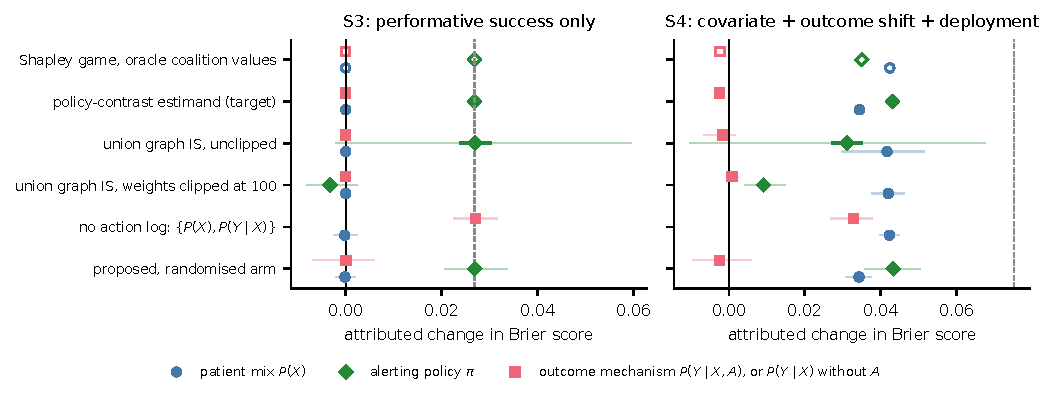
\includegraphics[width=0.8\textwidth]{figures/fig1_attribution.pdf}
\caption{Attribution of the Brier-score change under S3 and S4: two oracle
references (open markers: Shapley game; filled: policy-contrast estimand) and
four estimators. Means over 100 independent replicates ($n = 20{,}000$ per
environment); thick bars 95\% bootstrap intervals of the mean, thin bars the
central 95\% of single replicates. The monitor has no policy player. Dashed
line: total change.}\label{fig:attr}\end{figure*}

\paragraph{Two references, not one (Figure~\ref{fig:attr}).} With oracle
coalition values, the symmetric Shapley share of the policy player and the
policy-contrast estimand coincide under S3 ($+0.0269$ vs.\ $+0.0269$) and
differ under S4 ($+0.0351$ vs.\ $+0.0431$; Monte Carlo SEs below $10^{-4}$).
The marginal contributions of the policy player to $\emptyset$, $\{X\}$,
$\{Y\}$ and $\{X, Y\}$ are $+0.0269$, $+0.0431$, $+0.0273$ and $+0.0431$;
the difference between their average and the last is the interaction
$I(X, \pi) = +0.0162$, which Shapley symmetry halves ($I(\pi, Y) = +0.0004$): the exogenous mix shift pushes more patients above the alert
threshold, so the policy does more work in the shifted population, which is
the population in which the keep-or-retrain decision is taken. The
policy-contrast estimand conditions on it; the symmetric share does not
(Appendix~\ref{app:robustness}).

\paragraph{F1: misattribution is silent (Figure~\ref{fig:attr}).} Under S3 the
observed Brier score rises by $+0.0268$ [$+0.0264$, $+0.0273$]. Without action
logs the two-player game assigns $+0.0271$ [$+0.0266$, $+0.0275$] to
$P(Y \mid X)$ and $-0.0002$ [$-0.0004$, $+0.0000$] to $P(X)$: all of the
policy's contribution ($+0.0269$) is booked to the outcome mechanism,
precisely (single-run SD $0.0023$), and nothing in the monitor's output
signals a problem; its own bootstrap interval covers the marginal game it
estimates in $93\%$ of replicates and the policy-contrast outcome term in
$0\%$. The alert leaves a trace only for an analyst who looks for it: event
rates drop discontinuously at the alert threshold (Appendix~\ref{app:rd}).
The union-graph estimator is right on average ($+0.0270$ [$+0.0237$,
$+0.0305$]) but unusable in any single run (SD $0.017$, effective sample size
$107$ of $20{,}000$); clipping restores the variance and reverses the sign
($-0.0033$ [$-0.0040$, $-0.0027$]). The proposed decomposition recovers its
estimand, $+0.0269$ [$+0.0263$, $+0.0276$] from the randomised arm and
$+0.0268$ [$+0.0265$, $+0.0270$] with oracle policy weights, with
analyst-interval coverage of $95\%$. Under S1 and S2 all estimators agree with
their targets; under S4 the
randomised-arm estimate ($+0.0343 / -0.0025 / +0.0433$ for $X / Y / \pi$)
matches the target ($+0.0345 / -0.0024 / +0.0431$).

\begin{figure*}[t]\centering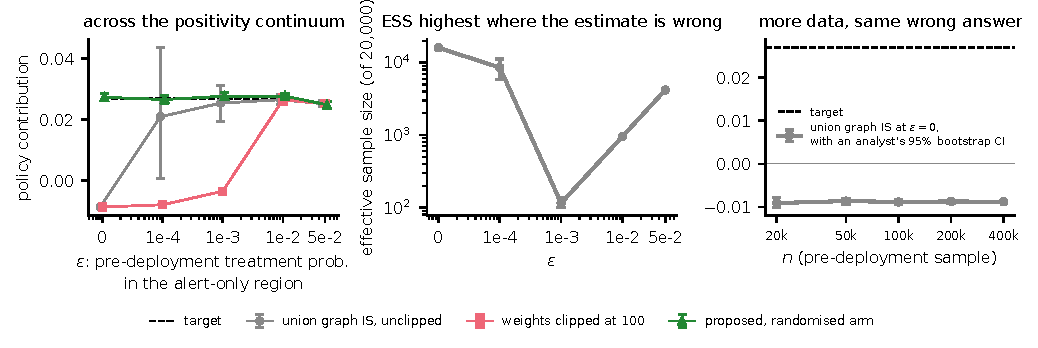
\includegraphics[width=0.8\textwidth]{figures/fig2_positivity.pdf}
\caption{The positivity continuum, S3 operating point. Left: policy
contribution by estimator as the pre-deployment treatment probability
$\varepsilon$ in the alert-only region varies (30 replicates per
$\varepsilon$). Middle: effective sample size of the policy weights. Right: at
$\varepsilon = 0$, the union-graph estimate against its target as $n$ grows;
bars are the median analyst's 95\% patient-level bootstrap interval, which
narrows around a value of the wrong sign.}\label{fig:positivity}\end{figure*}

\paragraph{F2: more data makes the wrong answer more confident
(Figure~\ref{fig:positivity}).} At $\varepsilon = 0$ the union-graph estimator
returns $-0.0088$ [$-0.0090$, $-0.0086$] against a target of $+0.0269$, with an
effective sample size of $15{,}993$ of $20{,}000$ and no extreme weight: the
pre-deployment sample contains no treated patient in the alert-only region, so
the estimator silently omits the cell, the usual consequence of a structural
positivity violation~\citep{petersen2012positivity}. Scaling $n$ from
$2 \times 10^4$ to $4 \times 10^5$ leaves the bias at $-133\%$ of the target
while an analyst's bootstrap interval narrows from [$-0.0102$, $-0.0077$] to
[$-0.0091$, $-0.0085$] and excludes the target in every replicate. Effective
sample size is not monotone in $\varepsilon$ and is highest where the
estimate is wrong: it measures the variance regime, not identifiability.
Clipping bias is confined to $\varepsilon \in [10^{-4}, 10^{-3}]$. The
proposed decomposition recovers its estimand at every $\varepsilon$, with
analyst-interval coverage between $93\%$ and $100\%$.

\begin{figure*}[t]\centering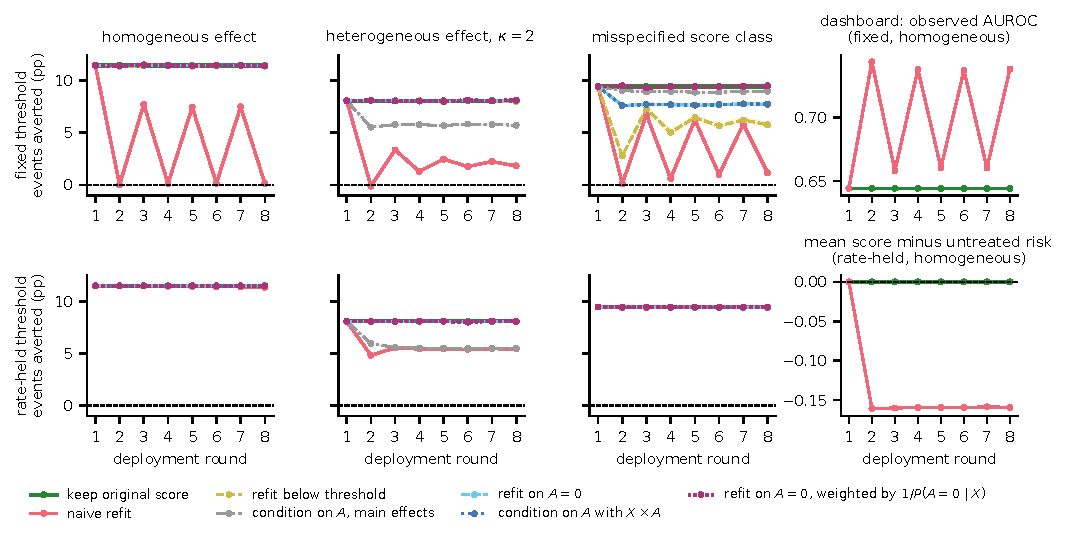
\includegraphics[width=0.68\textwidth]{figures/fig3_retrain.pdf}
\caption{Update rules after deployment (Experiment C), S3 operating point. Top:
fixed alert threshold; bottom: original alert rate held. First three columns
(one vertical scale): expected events averted against standard care for a
homogeneous effect, a heterogeneous effect ($\kappa=2$) and a misspecified
score class. Right column, naive refitting under a homogeneous effect:
observed AUROC in the deployed population (top, in antiphase with the benefit)
and mean score minus mean untreated risk (bottom, the calibration loss the
rate-held threshold hides). Fifty seeds per setting, eight rounds; bands are
95\% bootstrap intervals of the across-seed mean; dashed line standard
care.}\label{fig:retrain}\end{figure*}

\paragraph{F3: acting on the misattribution (Figure~\ref{fig:retrain}).}
A team that reads the monitor's attribution as outcome-mechanism drift refits
$f$ on post-deployment $(X, Y)$. The refit learns that the patients the alert
flagged are low risk, because their events were prevented, and stops flagging
them; the next round's data then contain their events again. We compare seven update rules over eight rounds against one
standard-care reference, under the deployed fixed threshold and with the
original alert rate held, for a homogeneous effect, a heterogeneous effect
($\kappa = 2$) and a misspecified score class (Appendix~\ref{app:retrain}).
Under the fixed threshold naive refitting fails in every setting; with a
homogeneous effect it enters the period-2 cycle of Theorem~1 of
\citet{liley2021model}: events averted fall from $11.46$ [$11.43$, $11.49$]
points to $0.01$ in round two and then alternate between about $7.5$ and
$0.1$, while observed AUROC is highest, $0.737$ to $0.744$ in the rounds in which
the alert averts almost nothing. Holding the alert rate removes the
loss under a homogeneous effect ($11.33$ [$11.27$, $11.39$] at round eight)
but hides a calibration loss, the refitted score lying $0.159$ below the
untreated risk, and under a heterogeneous effect keeps $5.42$ [$5.36$,
$5.48$] of $8.07$ points: holding the rate is a governance lever, not a fix.
The corrections form a hierarchy. Conditioning on the action with a single
treatment coefficient fails under heterogeneity ($5.72$ points); adding
treatment-by-covariate interactions restores $8.08$. Refitting below the
alert threshold needs no action log but keeps $5.77$ [$5.50$, $6.04$] of
$9.44$ points when the score class is misspecified. Refitting on untreated
patients, the observational counterpart of the holdout update of
\citet{liley2021model}, loses $1.71$ [$1.60$, $1.83$] points under
misspecification because the fit depends on which patients the current policy
leaves untreated; weighting them by the inverse probability of remaining
untreated~\citep{sperrin2018msm} removes that dependence and keeps the benefit
in all six settings ($9.50$ [$9.40$, $9.59$] misspecified, fixed threshold).
Every action-log correction assumes the logged covariates capture the
treatment decision. The loss scales with the events the action prevents: at
the MIMIC-IV event rate near $1\%$ naive refitting averts a sixth fewer
events than refitting on untreated patients and oscillates only in damped
form (F7).




% generated by sim2/make_tables.py; do not edit by hand
\begin{table}[t]
\centering\scriptsize
\setlength{\tabcolsep}{3pt}
\caption{Keep-or-refit rules, fixed alert threshold. Events averted against standard care in the window after the decision (percentage points), mean over 200 independent replicates per scenario; 95\% bootstrap intervals are within $\pm0.44$. Percentages give how often a rule refits. Regret is measured against the better of keeping and naive refitting in each replicate; a negative value beats both.}
\label{tab:decision}
\resizebox{\columnwidth}{!}{%
\begin{tabular}{lrrrrrr}
\toprule
Rule & S1 & S2 & S3 & S4 & \multicolumn{2}{c}{Regret}\\
& & & & & mean & worst\\
\midrule
Never refit & 15.4 & 12.6 & 11.5 & 16.6 & 1.0 & 4.2\\
Always refit (naive) & 10.8 & 16.8 & 0.0 & 5.1 & 6.9 & 11.5\\
Refit if exogenous share $>1/2$ & 10.8 (100\%) & 16.8 (100\%) & 11.5 (0\%) & 15.8 (8\%) & 1.4 & 4.6\\
Refit if outcome share $>1/2$ & 15.4 (0\%) & 16.8 (100\%) & 11.5 (0\%) & 16.6 (0\%) & 0.0 & 0.0\\
\quad same, monitor (no action log) & 15.4 (0\%) & 16.8 (100\%) & 0.0 (100\%) & 16.5 (1\%) & 2.9 & 11.5\\
Reference: refit on $A{=}0$ & 15.4 & 18.6 & 11.5 & 21.5 & $-$1.7 & $-$0.0\\
\bottomrule
\end{tabular}
}
\end{table}

\paragraph{F4: attribution-guided refitting (Table~\ref{tab:decision}).}
After the monitoring window of each scenario a rule keeps or naively refits
the score, and we count events in the next window (200 independent replicates
per scenario). Always refitting loses $11.5$ points in S3 and S4. Refitting
when the proposed decomposition assigns more than half of the change to
exogenous mechanisms never refits in S3, keeps the gain of refitting in S2
($16.8$ against $12.6$ points) and refits in $8\%$ of S4 replicates, but also
refits in S1, where the original
score is still the untreated risk, and costs $4.6$ points, because a naive
refit on standard-care data imports standard care's treatment of suspicious
patients. Mapping components to actions removes the loss: refitting only when
the outcome-mechanism term carries more than half of the change has zero
regret in all four scenarios at the calibrated operating point (at a $6.6\%$
event rate it loses $0.55$ points in S4; Appendix~\ref{app:robustness}).
Driven by the monitor without action logs, the same rule refits in S3 and
loses the whole benefit. With the alert rate held no two of the rules in
Table~\ref{tab:decision} differ by more than
$1.3$ points in S1 to S4; refitting on untreated patients, which needs
the action log rather than the randomised arm, matches the better of keeping
and naive refitting in S1 and S3 and beats both in S2 ($+1.7$) and S4
($+4.9$). Harm-weighted versions leave the ranking unchanged for harms up to
$0.2$ events per unnecessary treatment.

\paragraph{F5: deployment also moves the patient mix
(Figure~\ref{fig:triage}, Appendix~\ref{app:sites}).} A triage effect, a
covariate shift caused by deployment itself, breaks Assumption~\ref{ass:switch}
a second way: one event moves both $\pi$ and $P(X)$. The monitor books the
whole observed mix shift to $P(X)$, and so does the $X$ term of the proposed
decomposition; under a mixed shift the oracle Shapley target for $P(X)$
decreases with triage while the monitor's attribution increases. Two policy
estimands separate: the retrospective contrast (undo deployment, triage
included) grows from $+0.027$ to $+0.094$ as triage rises to $0.5$, the
prospective contrast (switch the alert off in the current mix), which the
keep-or-retrain decision needs, only to $+0.043$; the randomised arm recovers
the prospective one at every triage level (largest gap $0.0009$). Patient-level
randomisation cannot separate exogenous from deployment-caused mix shift,
because both arms draw from the post-deployment referral stream; a site
rollout can. In a stepped wedge with persistent sites (48 sites, six periods,
200 seeds per setting; Table~\ref{tab:sites}) a crossover difference in
differences recovers the retrospective term and the Brier-scale split of the
covariate shift when rollout order is random (biases within $2.1\%$), and a
site-cluster bootstrap gives nominal coverage. When early rollout goes
to sites whose characteristic also sets case mix and baseline risk, the
retrospective term is biased by $-10.5\%$ [$-11.5$, $-9.5$] even with common
covariate trends, and with site-specific trends the covariate-mean split is
biased as well ($+16.5\%$ induced, $-36.5\%$ exogenous): random rollout order, not site-level rollout as such,
identifies the split. Two qualifications carry over from cluster trials and
difference-in-differences with repeated cross-sections: randomising sites
does not separate the alert's effect from a change in who is enrolled after
randomisation~\citep{papadogeorgou2025selection}, and the deployment-caused
compositional change is here a target rather than a nuisance to be
removed~\citep{santanna2026compositional}; the experiment simulates a change
in the covariate distribution of patients who appear in the data, not
selection into the data (Section~\ref{sec:responsible}).

\paragraph{F6: discrimination and utility move in opposite directions
(Figure~\ref{fig:utility}, Appendix~\ref{app:intervals}).} Across treatment
effect and adherence, observed post-deployment AUROC falls monotonically (to
$0.637$ [$0.636$, $0.638$] at $\theta = 2.5$, adherence $0.9$), as expected
when treatment follows the prediction~\citep{pajouheshnia2017accounting},
while events averted rise to $12.2$ [$12.0$, $12.4$] points. Standard
decision-curve net benefit on observed outcomes falls from $+0.056$ [$+0.054$,
$+0.057$] to $-0.142$ [$-0.143$, $-0.141$]; net benefit against outcomes under standard care, which the
randomised arm identifies, is $+0.080$ at $\theta = 2.5$ for every adherence,
positive where standard decision-curve analysis is negative. The
pre-deployment AUROC ($0.745$) is itself below the AUROC against untreated
potential outcomes ($0.814$), because standard care already treats suspicious
patients: the baseline is not a clean measurement either. Charging each
unnecessary treatment a harm of $h$ events lowers events averted at adherence
$0.85$ from $11.50$ to $10.56$ points at $h = 0.1$ and $9.63$ at $h = 0.2$
(Table~\ref{tab:harm}).

\begin{figure*}[t]\centering
\IfFileExists{figures/fig7_mimic.pdf}{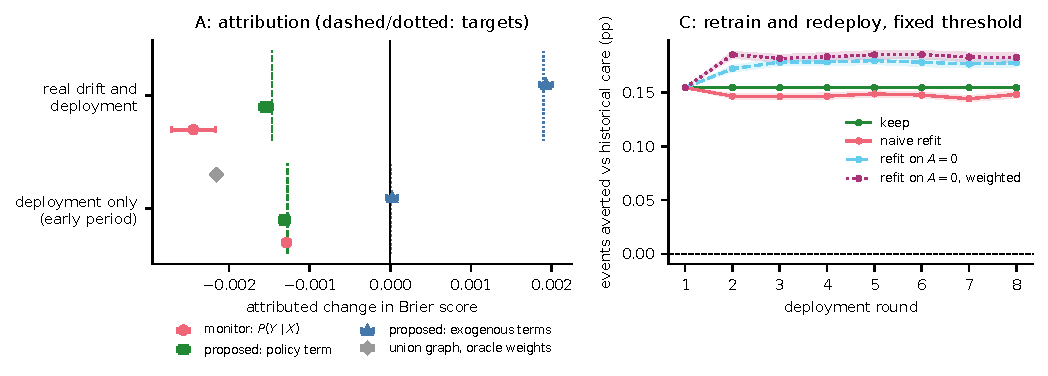
\includegraphics[width=0.8\textwidth]{figures/fig7_mimic.pdf}}{\fbox{\parbox{0.9\textwidth}{\centering Figure 7 is produced by \texttt{sim2/exp\_E6\_mimic.py} on credentialed MIMIC-IV data.}}}
\caption{Semi-synthetic MIMIC-IV. Real covariates and outcomes; simulated
deployment, clinician response, treatment effect and randomised arm (listed
in the text). Left: attribution of the Brier-score change when only the
deployment changes (early period before and after) and with real drift
between periods; dashed and dotted lines mark the policy and exogenous
targets. Right: events averted against historical care by four update rules
under the fixed threshold. Points are means over 200 (left) and 50 (right)
replicates that resample patients and redraw the simulated components; bars
and bands are 95\% bootstrap intervals over replicates.}\label{fig:mimic}\end{figure*}

\paragraph{F7: semi-synthetic MIMIC-IV (Figure~\ref{fig:mimic}).} We repeat
Experiments A and C on a ward-deterioration cohort from
MIMIC-IV~\citep{johnson2023mimic}: $368{,}995$ admissions of $155{,}852$
adult ward patients. Real: covariates (demographics, admission type, time
since admission, eleven routine blood tests), the outcome under historical
care (ICU admission or death within 12 hours; $0.84\%$ of admissions before
deployment, $1.04\%$ after) and the period (anchor years 2008--2013 against
2014--2019). Simulated: a logistic score fitted to part of the early period,
a $10\%$ alert rate, clinician response $0.85$, an action that prevents an
event with probability $0.5$ and causes none, a $30\%$ randomised arm and the
refit loop (Appendix~\ref{app:mimic}). No pre-deployment patient received the
action, so the union-graph estimator faces the $\varepsilon = 0$ failure of
F2; because the action only prevents events, the policy term is known exactly
for the finite cohort. Alerted patients have a mean predicted risk of $0.03$,
so preventing their events lowers the Brier score (the derivative of
$\E[(r - Y)^2]$ in $P(Y{=}1)$ is $1 - 2r$) and the monitor books an apparent
improvement to the outcome mechanism. With deployment only, the policy
contrast is $-0.00127$; the monitor books $-0.00128$ [$-0.00133$, $-0.00123$]
to $P(Y \mid X)$ and nothing to $P(X)$, while observed AUROC falls by $0.044$
and observed over expected events fall from $1.04$ to $0.87$. The randomised
arm estimates $-0.00131$ [$-0.00138$, $-0.00124$] (single-run SD $0.0005$
over about $138{,}000$ post-deployment admissions); the union-graph estimator
with oracle weights returns $-0.00215$ [$-0.00217$, $-0.00214$] whether the
action prevents $25\%$,
$50\%$ or $75\%$ of events (Table~\ref{tab:mimic-sens}), since with no
treated pre-deployment patient it cannot see the action. Between the periods
the Brier score rises by $+0.00190$ under historical care; with the alert
deployed the observed change is $+0.00039$, because the policy contrast,
$-0.00147$, hides $77\%$ of the deterioration. The randomised arm estimates
$-0.00154$ [$-0.00162$, $-0.00146$] and the exogenous change $+0.00193$
[$+0.00186$, $+0.00201$]; the monitor assigns $-0.00244$ [$-0.00272$,
$-0.00216$], the alert's effect included, to $P(Y \mid X)$. Under the fixed
threshold, events averted at round eight are $0.154$ points for the kept
score, $0.148$ [$0.145$, $0.152$] after naive refitting, $0.177$ [$0.173$,
$0.181$] after refitting on untreated patients and $0.183$ [$0.178$, $0.187$]
after the weighted refit: the naive refit learns the
prevented events and flags $10.7\%$ of patients against $15.4\%$, a damped
form of the cycle of F3, and the dashboard again ranks the rules in reverse.

\section{Related work}
\label{sec:related}

\paragraph{Attributing performance change.} \citet{zhang2023attributing}
attribute a performance change to distribution shifts with a cooperative game
over the mechanisms of a causal factorisation, valued by Shapley values and
estimated by importance weighting; \citet{quintasmartinez2024multiply} give
multiply robust estimators of the same game, consistent if either the density
ratios or the regression functions are correctly specified. That robustness
is to nuisance misspecification, not to the support failure of
Proposition~\ref{prop:absence}, which leaves the coalition value itself
undetermined by pre-deployment data. \citet{budhathoki2021rootcauses},
\citet{cai2023disde}, \citet{singh2024hierarchical} and
\citet{gordaliza2025causal} attribute distribution or performance change to
covariate and outcome-conditional mechanisms; all treat every mechanism as
exogenous to the audited model.

\paragraph{Performativity and model updating.} \citet{perdomo2020performative}
formalise performative prediction and analyse repeated retraining;
\citet{kabra2024limitations} show that naive retraining can be provably
suboptimal, and \citet{lee2026partially} let the distribution respond both to
the model and to exogenous drift. For clinical risk scores,
\citet{liley2021model} show that naive updating converges to a score that
predicts its own effect or oscillates, and propose a holdout set whose size
\citet{haidarwehbe2025holdout} optimise. \citet{boeken2024evaluating} treat
deployment of a decision support system as a causal domain shift and identify
deployment and retraining effects under absolute continuity, assuming
deployment leaves the covariate distribution unchanged. We use the holdout
device for attribution, their absolute-continuity condition to locate where
the game loses identification, and a site-level design to separate the
deployment-caused covariate shift their assumptions exclude.

\paragraph{Prediction under interventions, monitoring, deployed alerts.}
Estimands for a model whose predictions trigger treatment are defined by
\citet{sperrin2018msm}, \citet{vangeloven2020prediction},
\citet{lin2021scoping}, \citet{keogh2024prediction} and
\citet{luijken2024estimands}; treatment use biases
validation~\citep{pajouheshnia2017accounting}, standard metrics do not measure
the outcome reduction a model brings~\citep{schuler2020performance}, and an
accurate model can harm through self-fulfilling prophecies while its
discrimination stays intact~\citep{vanamsterdam2025selffulfilling}.
\citet{feng2024designing} compare monitoring strategies under performativity,
effective interventions confound post-market
surveillance~\citep{ansari2025challenges}, feedback-aware monitors inject
randomisation or weight~\citep{corbin2023avoiding, kim2025monitoring} or
monitor conditional performance~\citep{feng2024monitoring, guan2026detecting},
\citet{gowerwinter2025performative} test whether a detected concept drift is
performative or intrinsic, and regulatory work covers device
updates~\citep{wu2024regulating, gonzalez2024regulating, afdideh2026aegis};
these works detect, estimate or govern a change but do not attribute it to
mechanisms. Evaluations of deployed alerts use the designs of
Section~\ref{sec:ident} to estimate the alert's effect on outcomes:
patient-level~\citep{wilson2021aki} and unit-level
randomisation~\citep{rossetti2025concern}, a staggered
rollout~\citep{escobar2020automated} and a threshold regression
discontinuity~\citep{gallo2024effectiveness}; we use the same designs to
identify the alert's share of a monitored performance change.

\section{Limitations and responsible-use statement}
\label{sec:responsible}

\paragraph{Limitations.} Results are theoretical and synthetic, or
semi-synthetic where MIMIC-IV covariates, outcomes and temporal drift are used
with a simulated deployment; no real deployment logs are analysed. On MIMIC-IV
the alert and its effect are simulated, the periods are anchor-year groups
that date an admission only to within several years, and the split of the
real drift into covariate and outcome terms has no ground truth. The
calibrated operating point is deliberately strong (an acted-upon alert cuts
the odds of the event by about 12, $28\%$ of patients are flagged only by the
alert, the untreated event rate is about $40\%$); magnitudes scale with these
choices while the direction of the misattribution does not
(Proposition~\ref{prop:misattr}; Table~\ref{tab:prevalence}; F7). The
decomposition is order-dependent in its split of interaction terms, the
threshold discontinuity identifies only a local effect, and a randomised
unalerted arm assumes no interference between arms, which shared ward staff,
alert fatigue and clinicians' learning can violate. Deployment-caused
covariate shift is modelled as a change in the distribution of patients who
reach the data; if deployment also changes who is admitted, referred or
recorded, the outcomes of excluded patients are missing, a selection problem
that neither the randomised arm nor the site designs
address~\citep{papadogeorgou2025selection}.

\paragraph{Responsible use.} From routine observational post-deployment data,
model-mediated improvement is not identifiable; an attribution produced
without a source of identifying variation is a sensitivity analysis, not
evidence. Misattribution has a clinical cost in both directions: attributing
performative success to outcome-mechanism shift retrains an effective model
and removes its benefit; attributing a genuine outcome shift to the model's
success leaves a degraded model in place (F7). A randomised unalerted
arm withholds a possibly beneficial alert from some patients; its size trades
that cost against the precision of the
attribution~\citep{haidarwehbe2025holdout}, steeply at ward-deterioration
event rates (F7). The method requires logging of alert
exposure and action, to be governed under existing post-market surveillance
frameworks~\citep{gonzalez2024regulating}; nothing here supports deploying
or retaining a model without prospective evaluation of patient outcomes.

\bibliography{references}

\appendix
\section{Information budget}
\label{app:information}
\begin{table*}[t]
\centering\small
\caption{Information budget for every estimator and update rule reported.
``Pre'' and ``post'' mean observed samples; $A$ is the recorded action.
Oracle rows (last column ``Yes'') use true simulator mechanism probabilities
and serve only to validate targets. The original deployed score is available
to every method. Site designs also need site identities and rollout dates;
the plug-in Brier-scale $X$ split of the site-rollout experiment additionally assumes a Gaussian
location shift. The weighted refit needs the alert exposure and the
clinician-response probabilities, logged or estimated.}
\label{tab:information}
\begin{tabular}{llllll}
\toprule
Estimator or rule & Pre sample & Post sample & Action log & Randomised arm & Oracle\\
\midrule
\multicolumn{6}{l}{\emph{Attribution (Experiments A, B and F, site rollout, MIMIC-IV)}}\\
Monitor, two-player, estimated ratio & $(X,Y)$ & $(X,Y)$ & No & No & No\\
Monitor, two-player, oracle ratios & $(X,Y)$ & None & No & No & Yes\\
Union graph IS, raw or clipped & $(X,A,Y)$ & None & Yes & No & Yes\\
Proposed, randomised arm & $(X,Y)$ & $(X,Y)$ & No & Yes & No\\
Proposed, oracle policy weights & $(X,Y)$ & $(X,A,Y)$ & Yes & No & Yes\\
Site crossover difference in differences & $(X,Y)$ & $(X,Y)$ & No & No & No\\
Threshold discontinuity, local ITT & None & $(\rhat,Y)$ & No & No & No\\
\multicolumn{6}{l}{\emph{Update rules (Experiment C) and keep-or-refit decisions}}\\
Naive refit & Score only & $(X,Y)$ & No & No & No\\
Refit below the alert threshold & Score only & $(X,Y)$, alert & No & No & No\\
Refit on $A=0$; condition on $A$ & Score only & $(X,A,Y)$ & Yes & No & No\\
Refit on $A=0$, weighted & Score only & $(X,A,Y)$, alert & Yes & No & No\\
Attribution-guided refit & \multicolumn{5}{l}{that of the attribution driving it}\\
\bottomrule
\end{tabular}
\end{table*}
The oracle rows validate targets in simulation. They are not deployable
estimators. The randomised-arm row uses assignment and outcome, while the site
row needs a credible site-level comparison; neither observes counterfactual
outcomes directly.

\section{Threshold-discontinuity experiment}
\label{app:rd}
On the intention-to-treat scale the local jump at $\tau_r$ is $-0.332$
[$-0.338$, $-0.326$], against an average policy effect of $-0.291$ among the
alerted, which it overstates by $14\%$; the effect curve is hump-shaped and
falls to zero at high scores, where standard care already treats.

\begin{proposition}[Local-to-global gap under threshold discontinuity]
\label{prop:rd}
Let the alert fire when $\rhat \geq \tau$, let $\pi_1 = \pi_0$ below $\tau$,
and let $\theta(r) = \E[Y(\pi_1) - Y(\pi_0) \mid \rhat = r]$ be the
intention-to-treat effect curve of the alert on the event probability, with
$F$ the distribution of $\rhat$ after deployment and
$\bar F(\tau) = P(\rhat \geq \tau)$. If $\E[Y(\pi_0) \mid \rhat = r]$ is
continuous at $\tau$, the post-deployment jump
$\lim_{r \downarrow \tau} \E[Y \mid \rhat = r] -
\lim_{r \uparrow \tau} \E[Y \mid \rhat = r]$ identifies $\theta(\tau)$. The
policy's effect on the event rate is
$\Theta = \int_{r \geq \tau} \theta(r)\, dF(r)$, and for the Brier score the
policy term of~\eqref{eq:decomp} is
$\Delta_\pi = \int_{r \geq \tau} (1 - 2r)\, \theta(r)\, dF(r)$; the
discontinuity alone identifies neither. (a) If $\theta$ is constant on
$[\tau, 1]$, then $\Theta = \theta(\tau)\, \bar F(\tau)$ and
$\Delta_\pi = \theta(\tau) \int_{r \geq \tau} (1 - 2r)\, dF(r)$. (b) If $\theta$
has constant sign and $|\theta|$ is monotone on $[\tau, 1]$, then
$|\theta(\tau)|\, \bar F(\tau)$ bounds $|\Theta|$ from below when the effect
grows with the score and from above when it shrinks.
\end{proposition}

\noindent\emph{Reading.} The first statement is standard regression-discontinuity
identification, which \citet{gallo2024effectiveness} use to evaluate a deployed
deterioration alert. The proposition adds the gap between that local effect and
the two global quantities, and the weight $1 - 2r$ that separates the
Brier-scale term from the effect on the event rate; closing the gap away from
the threshold needs assumptions beyond continuity, such as the conditional
independence of \citet{angrist2015wanna}. Which case applies is a clinical
question: the effect shrinks above the threshold when standard care already
treats most high-score patients. In our simulation the curve is neither constant nor monotone: the
effect strengthens from $-0.34$ just above the threshold to $-0.42$, then
fades to near zero at high scores, and the local jump overstates the average
effect among alerted patients by $14\%$ (below).

At the S3 operating point, each of 40 replicates draws $80{,}000$
post-deployment patients and fits a local linear regression of the observed
outcome on $\rhat - \tau_r$, with separate slopes on each side of the
threshold, within a bandwidth of $0.04$. The jump is an intention-to-treat
effect: it compares alerted with unalerted patients at the threshold, whatever
treatment they then received. It estimates $\theta(\tau_r)$ as $-0.332$
[$-0.338$, $-0.326$], while the average policy effect among alerted patients,
$\E[Y(\pi_1) - Y(\pi_0) \mid \rhat \geq \tau_r]$ from the simulator's potential
outcomes, is $-0.291$. Both are smaller than the effect of treatment against no
treatment among the alerted ($-0.405$): suspicious patients near the threshold
are treated under both policies, and only $85\%$ of alerts are acted on. The
effect curve $\theta(r)$, averaged in 12 score bins from $0.45$ to $0.95$,
strengthens from $-0.34$ just above the threshold to $-0.42$ near
$\rhat = 0.64$, because a fixed logit effect removes more probability at
higher baseline risk, then fades to $-0.07$ near $0.85$ and to about zero above
$0.87$, because standard care already treats most high-score patients. Neither
condition of Proposition~\ref{prop:rd} holds, and the local jump overstates the
average effect by $14\%$.

Figure~\ref{fig:rd} shows the curve and its Brier-scale weighting.
Integrated against the score distribution, the curve gives the policy's effect
on the event rate, $\Theta = -0.1150$, and with weight $1 - 2r$ the
Brier-scale policy term, $+0.0269$ [$+0.0269$, $+0.0270$], the policy contrast
of F1. Extrapolating the local jump as a constant effect
(Proposition~\ref{prop:rd}(a)) gives $+0.0461$ [$+0.0452$, $+0.0470$],
$71\%$ too large: the weight $1 - 2r$ is largest in magnitude at high scores,
where the effect has faded.

\begin{figure*}[t]\centering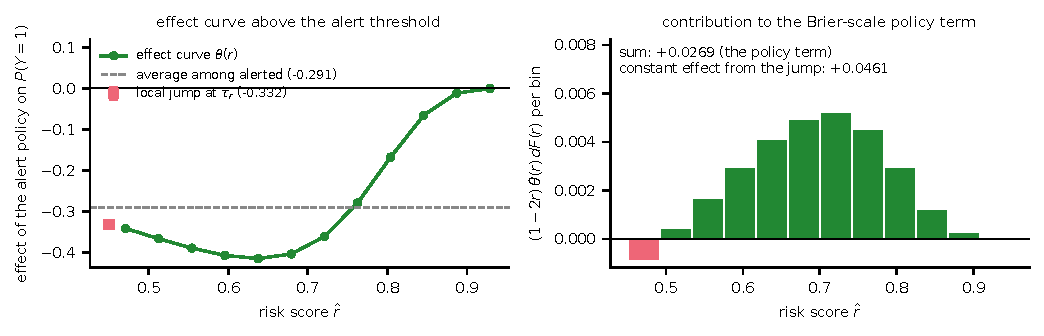
\includegraphics[width=\textwidth]{figures/fig_rd_curve.pdf}
\caption{Threshold-discontinuity experiment, S3 operating point, 40
independent replicates of $80{,}000$ post-deployment patients. Left: the alert
policy's effect on the event probability by score bin (95\% bootstrap bands
over replicates, narrower than the line), its average among alerted patients,
and the local jump at the threshold. Right: each bin's contribution
$(1 - 2r)\,\theta(r)\,dF(r)$ to the Brier-scale policy term; the bins sum to
the policy term, while a constant effect equal to the local jump would give the
second value shown.}\label{fig:rd}\end{figure*}

\section{Robustness of Experiments A and B}
\label{app:robustness}
\paragraph{Ordering dependence of the policy share.} Under S4 the marginal
contributions of the policy player to $\emptyset$, $\{X\}$, $\{Y\}$ and
$\{X, Y\}$ are $+0.0269$, $+0.0431$, $+0.0273$ and $+0.0431$; the symmetric
Shapley value averages them ($+0.0351$), the policy-last ordering takes the
last ($+0.0431$), and the spread between orderings is the interaction
$I(X, \pi) = +0.0162$ reported in the main text.

The deployed score remains logistic-linear. Additional covariates enter the
linear score, and in the misspecified cells the true outcome logit also includes
$0.65\{X_1X_3+0.3(X_3^2-1)\}$. Experiment A repeats S1--S4; Experiment B
repeats the positivity continuum and an independent sample-size sweep at
$\varepsilon=0$. Each row uses an independent seed block, 12 replications of
$12{,}000$ patients per environment, and a $120{,}000$-patient oracle reference.

% generated by sim2/make_tables.py; do not edit by hand
\begin{table}[h]
\centering\scriptsize
\caption{S3 attribution and $\varepsilon=0$ bias with more covariates and a misspecified outcome, Brier units. Estimates are means over 12 independent seeds with 95\% bootstrap intervals. The union-graph bias at $n=96{,}000$ is relative to its oracle Shapley target.}
\label{tab:robustness}
\resizebox{\columnwidth}{!}{%
\begin{tabular}{lrrrr}
\toprule
Setting & True $\Delta R$ & Monitor $Y|X$ & Proposed $\pi$ & Union bias\\
\midrule
$d=10$, linear & 0.0313 & 0.0310 [0.0297, 0.0321] & 0.0310 [0.0284, 0.0339] & $-$0.0396 [$-$0.0398, $-$0.0394]\\
$d=10$, nonlinear & 0.0280 & 0.0264 [0.0245, 0.0282] & 0.0283 [0.0259, 0.0308] & $-$0.0364 [$-$0.0367, $-$0.0362]\\
$d=20$, linear & 0.0311 & 0.0306 [0.0287, 0.0324] & 0.0315 [0.0287, 0.0343] & $-$0.0401 [$-$0.0402, $-$0.0399]\\
$d=20$, nonlinear & 0.0286 & 0.0279 [0.0262, 0.0295] & 0.0290 [0.0248, 0.0330] & $-$0.0362 [$-$0.0364, $-$0.0360]\\
\bottomrule
\end{tabular}
}
\end{table}

F1 survives in all four settings: with no action player, nearly the entire S3
change is booked to the marginal outcome mechanism. F2 also survives: the
$\varepsilon=0$ union-graph bias remains between $-0.036$ and $-0.040$ as
sample size rises from $6{,}000$ to $96{,}000$; the full independent-seed
sweeps and all S1--S4 results are in \texttt{merged\_expAB\_robustness.json}.
F3 under a misspecified score class is covered by Experiment C (Appendix~\ref{app:retrain}).

\paragraph{Prevalence.} The calibrated operating point has an untreated event
rate near $40\%$, so alerted patients mostly have predicted risk above $0.5$
and preventing their events raises the Brier score; the derivative of
$\E[(r - Y)^2]$ in $P(Y{=}1)$ is $1 - 2r$. Table~\ref{tab:prevalence} lowers
the outcome intercept with the alert rate held at $20\%$. At event rates of
$14\%$ and $7\%$ the same deployment lowers the Brier score ($-0.0076$ and
$-0.0065$) while observed AUROC still falls, and the monitor again books the
whole change to $P(Y \mid X)$. F1 survives at every prevalence, but at
realistic ward-deterioration prevalence a successful alert shows up as an
apparent improvement of the outcome mechanism, not as a drop. The MIMIC-IV
cohort (last row of Table~\ref{tab:prevalence}) shows this on real covariates
and outcomes: at an event rate of $0.85\%$ the deployment lowers the Brier
score by $0.0013$ while AUROC falls from $0.747$ to $0.702$, and the monitor
books the whole change to $P(Y \mid X)$.

% generated by sim2/make_tables.py; do not edit by hand
\begin{table}[h]
\centering\scriptsize
\setlength{\tabcolsep}{3pt}
\caption{Sign of the S3 change across outcome prevalence, alert rate held at 20\%. Oracle values (expected Brier scores, mean over 4 independent blocks of 400{,}000 patients; Monte Carlo SE below $10^{-4}$). The monitor books the whole change to $P(Y\mid X)$ at every prevalence; only its sign changes. Last row: deployment only in the semi-synthetic MIMIC-IV experiment (Appendix~\ref{app:mimic}; alert rate 10\%, 138{,}278 held-out early-period admissions), exact in expectation over the simulated components; its monitor term is the mean of the estimator over 200 replicates.}
\label{tab:prevalence}
\resizebox{\columnwidth}{!}{%
\begin{tabular}{rrrrrr}
\toprule
Event rate & Mean score, alerted & $\Delta R$ & Policy (Shapley) & Monitor $Y|X$ & AUROC before, after\\
\midrule
0.395 & 0.80 & $+$0.0187 & $+$0.0187 & $+$0.0187 & 0.745, 0.694\\
0.254 & 0.63 & $+$0.0023 & $+$0.0023 & $+$0.0023 & 0.744, 0.697\\
0.137 & 0.40 & $-$0.0076 & $-$0.0076 & $-$0.0075 & 0.748, 0.707\\
0.066 & 0.22 & $-$0.0065 & $-$0.0065 & $-$0.0065 & 0.754, 0.719\\
\midrule
0.008 & 0.03 & $-$0.0013 & $-$0.0013 & $-$0.0013 & 0.747, 0.702\\
\bottomrule
\end{tabular}
}
\end{table}

Table~\ref{tab:prevalence-est} repeats Experiment A and the keep-or-refit rules with estimators at an
untreated event rate of $6.6\%$ (alert rate $20\%$). Under S3 the monitor
books $-0.0065$ [$-0.0068$, $-0.0062$] to $P(Y \mid X)$, and its interval
covers the policy-contrast outcome term, zero, in $2\%$ of replicates; the
randomised arm recovers the policy term with $96\%$ coverage. Under S4 the
policy term ($-0.0178$) offsets most of the outcome-mechanism shift
($+0.0242$): the monitor books $+0.0098$ [$+0.0094$, $+0.0103$] to
$P(Y \mid X)$, so a successful alert hides a real deterioration. Among the keep-or-refit rules the
monitor-driven outcome rule refits in every S3 replicate and keeps $0.02$ of
the $0.91$ points that keeping the score retains; the outcome-share rule
loses $0.55$ points in S4, where the oracle outcome share ($0.52$) sits at the
cut-off; refitting on untreated patients matches the better of keeping and
naive refitting in S1 and S3 and beats both in S2 and S4.

% generated by sim2/make_tables.py; do not edit by hand
\begin{table*}[t]
\centering\scriptsize
\caption{Experiment A and the keep-or-refit rules at an untreated event rate of 6.6\% ($b_0 = -3.5$, alert rate 20\%), $n = 20{,}000$ per environment. Top: attribution of the Brier-score change, oracle targets and estimator means with 95\% bootstrap intervals over 100 replicates, and coverage (\%) of the 95\% patient-level bootstrap interval: the proposed policy term against its target, and the monitor's $P(Y\mid X)$ term against the policy-contrast outcome term. The union-graph estimator targets the policy player's Shapley value, $-$0.0065 in S3 and $-$0.0117 in S4. Bottom: keep-or-refit rules, events averted after the keep-or-refit decision (percentage points, fixed threshold, 200 replicates per scenario), with how often a rule refits.}
\label{tab:prevalence-est}
\resizebox{\textwidth}{!}{%
\begin{tabular}{lcccccc}
\toprule
Scenario & $\Delta R$ & Policy contrast & Monitor $P(Y\mid X)$ & Proposed $\pi$ & Union graph $\pi$ & Coverage: proposed, monitor\\
\midrule
S3 & $-$0.0065 & $-$0.0065 & $-$0.0065 [$-$0.0068, $-$0.0062] & $-$0.0065 [$-$0.0070, $-$0.0060] & $-$0.0062 [$-$0.0071, $-$0.0050] & 96, 2\\
S4 & $+$0.0469 & $-$0.0178 & $+$0.0098 [$+$0.0094, $+$0.0103] & $-$0.0176 [$-$0.0182, $-$0.0170] & $-$0.0111 [$-$0.0126, $-$0.0093] & 96, 0\\
\bottomrule
\end{tabular}
}

\vspace{0.6em}
\begin{tabular}{lcccc}
\toprule
Rule & S1 & S2 & S3 & S4\\
\midrule
Never refit & 1.59 & 1.47 & 0.91 & 2.54\\
Always refit (naive) & 0.56 & 1.95 & 0.02 & 1.61\\
Refit if exogenous share $>1/2$ & 0.56 (100\%) & 1.95 (100\%) & 0.86 (6\%) & 1.61 (100\%)\\
Refit if outcome share $>1/2$ & 1.59 (0\%) & 1.95 (100\%) & 0.85 (6\%) & 1.99 (57\%)\\
\quad same, monitor (no action log) & 1.59 (0\%) & 1.95 (100\%) & 0.02 (100\%) & 2.54 (0\%)\\
Reference: refit on $A{=}0$ & 1.58 & 2.69 & 0.92 & 4.06\\
\bottomrule
\end{tabular}
\end{table*}


\begin{figure*}[t]\centering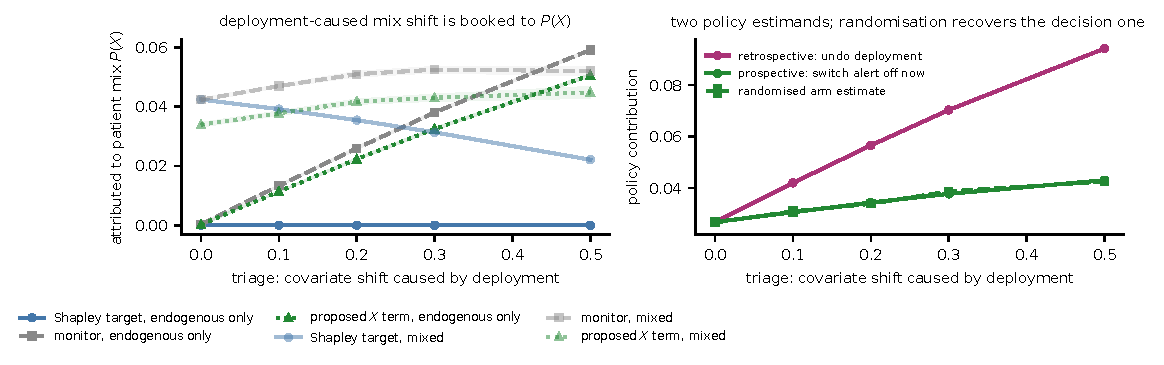
\includegraphics[width=\textwidth]{figures/fig4_triage.pdf}
\caption{Deployment-caused covariate shift (triage), 30 independent
replicates per triage level. Left: attribution to $P(X)$ by the oracle Shapley
target, the monitor and the proposed $X$ term, for a deployment-only and a
mixed shift, with 95\% bootstrap bands of the mean. Right: retrospective and
prospective policy contrasts (oracle) and the randomised-arm estimate with
95\% bootstrap intervals.}\label{fig:triage}\end{figure*}

\section{Persistent-site stepped wedge}
\label{app:sites}
The site-rollout experiment follows 48 sites for six periods. Four cohorts of 12 sites cross
at periods 2--5; the period-5 cohort supplies not-yet-deployed controls for the
three earlier crossovers. A fixed site characteristic $z$ shifts the site's
covariate mean by $0.5z$ and its outcome logit by $0.4z$. Rollout priority is
random, or $0.85z$ plus noise (correlation between early rollout and $z$ about
$0.78$); the covariate trend is common ($0.1$ per period) or site specific
($0.1 + 0.04z$ per period). Deployment adds a triage shift of $0.25$ to each
covariate. A difference in differences of observed Brier losses against
not-yet-deployed sites estimates the retrospective term at crossover, and the
controls' mean covariate change gives the exogenous increment of the
covariate-mean split. Two Brier-scale split estimators are compared. The
plug-in estimator reweights the switching site's pre-rollout losses under a
Gaussian location shift, to the controls' average covariate shift for the
exogenous part and to the site's own shift for the total. The DiD-anchored
estimator takes the exogenous part from the controls' observed loss change
and the deployment-caused part as the reweighted loss change at the site's
own shift minus that control change. Simulator counterfactuals are used only
to measure bias.

% generated by sim2/make_tables.py; do not edit by hand
\begin{table*}[t]
\centering\scriptsize
\caption{Persistent-site stepped wedge: bias as a percentage of the true value, with 95\% bootstrap interval, over 200 independent seeds per row. Rollout order is random or linked to the site characteristic; covariate trends are common or site specific. Retrospective term: crossover difference in differences. $X$ split in the covariate mean, and on the Brier scale by the plug-in and the DiD-anchored estimators.}
\label{tab:sites}
\resizebox{\textwidth}{!}{%
\begin{tabular}{lccccccc}
\toprule
Rollout order, trend & Retrospective & \multicolumn{2}{c}{$X$ mean split} & \multicolumn{2}{c}{Brier $X$ split, plug-in} & \multicolumn{2}{c}{Brier $X$ split, DiD-anchored}\\
\cmidrule(lr){3-4}\cmidrule(lr){5-6}\cmidrule(lr){7-8}
 & Retro. & Induced & Exog. & Induced & Exog. & Induced & Exog.\\
\midrule
Random, common & $-$0.2 [$-$1.3, $+$0.9] & $+$0.3 [$-$0.2, $+$0.9] & $-$0.3 [$-$0.9, $+$0.3] & $+$0.2 [$-$1.0, $+$1.4] & $-$0.6 [$-$1.6, $+$0.4] & $-$1.0 [$-$3.0, $+$1.0] & $+$2.1 [$-$1.4, $+$5.6]\\
Random, site-specific & $-$0.7 [$-$1.7, $+$0.4] & $-$0.3 [$-$1.1, $+$0.5] & $+$0.3 [$-$1.2, $+$1.8] & $-$15.2 [$-$16.7, $-$13.6] & $+$46.7 [$+$44.2, $+$49.2] & $-$0.6 [$-$3.1, $+$2.1] & $+$1.6 [$-$5.0, $+$8.5]\\
Linked, common & $-$10.5 [$-$11.5, $-$9.5] & $-$0.1 [$-$0.7, $+$0.5] & $+$0.3 [$-$0.4, $+$1.1] & $+$1.6 [$-$0.3, $+$3.5] & $+$1.0 [$-$0.6, $+$2.6] & $-$40.0 [$-$42.8, $-$37.2] & $+$81.9 [$+$77.8, $+$85.9]\\
Linked, site-specific & $-$5.6 [$-$6.6, $-$4.5] & $+$16.5 [$+$15.8, $+$17.1] & $-$36.5 [$-$37.4, $-$35.6] & $+$9.5 [$+$7.3, $+$11.9] & $-$17.4 [$-$19.9, $-$14.7] & $-$24.2 [$-$27.2, $-$21.0] & $+$59.7 [$+$54.3, $+$65.2]\\
\bottomrule
\end{tabular}
}
\end{table*}

With random rollout order every estimate is unbiased except the plug-in split
under site-specific trends ($+47\%$ exogenous, $-15\%$ induced), which imputes
the average trend into each site's loss although the loss responds to a trend
differently at sites with different $z$. With order linked to $z$, the
retrospective difference in differences is biased ($-10.5\%$ with common
trends, $-5.6\%$ with site-specific ones), because parallel covariate trends do
not produce parallel Brier trends when baseline risk differs, and the
DiD-anchored split inherits that bias; the plug-in split is unbiased with
common trends, where its location model holds at every site. No estimator is
unbiased in the linked, site-specific cell. These results concern the
crossover cohorts with a not-yet-deployed comparison; the last cohort's effect
is not identified without an additional period or assumption.

\emph{Intervals that respect the design.} The bootstrap intervals of
Table~\ref{tab:sites} are over independent realisations of the wedge and
measure Monte Carlo error. An analyst holds one realisation, in which patients
are nested in sites and sites persist across periods, so the analyst's
interval must resample sites, not patients. For each of 100 independent
realisations per row we resample sites with replacement within each rollout
cohort (300 resamples), recompute the retrospective difference in differences
and the DiD-anchored split, and ask whether the 95\% percentile interval
covers that realisation's simulator value
(\texttt{sim2/exp\_G2\_sites\_clusterboot.py},
\texttt{merged\_expG2\_clusterboot.json}). Under random rollout order the
site-cluster interval covers the retrospective term in $98\%$ and $99\%$ of
realisations and the deployment-caused split in $100\%$, with a bootstrap
standard deviation between $0.84$ and $0.99$ of the across-realisation one;
the exogenous part is covered in $93\%$ and $87\%$, the last with only the
late cohort as control. Under rollout order linked to $z$ coverage falls to
$82\%$ and $64\%$ for the retrospective term and the deployment-caused split
with common trends, and to $13\%$ for the exogenous part: a design-respecting
interval reports the sampling uncertainty of a biased estimator and cannot
repair the parallel-trends failure.

\section{Update rules after deployment (Experiment C)}
\label{app:retrain}
Each seed draws an evaluation population and an independent calibration
population of $20{,}000$ patients, and in each round a training sample of
$8{,}000$ patients treated under the current rule; all rules share these draws
(common random numbers), and each of the six settings has its own seed block
of 50 seeds. Events are expected values on the evaluation population, without
outcome noise, against standard care on the same population. The
heterogeneous effect is $\theta + \kappa (X_2 - X_1)/\sqrt{2}$ on the logit
scale; at $\kappa = 2$ the action is harmful for about $11\%$ of patients. The
misspecified truth adds the term of Appendix~\ref{app:robustness}, $0.65\{X_1X_2 + 0.3(X_2^2 - 1)\}$ to the
untreated logit; there the original score is the population-best logistic
approximation to the untreated risk, so a correct and stable update
reproduces it. The weighted refit uses $1/P(A = 0 \mid X)$ from the alert rule
and the response probabilities ($0.8$ for suspicious patients, $0.85$ for
alerted others, $\varepsilon$ otherwise). Estimating $P(A = 1 \mid X)$ instead,
by a logistic regression of $A$ on $X$, the alert and their interaction, changes
round-eight events averted by at most $0.01$ points in any setting.

% generated by sim2/make_tables.py; do not edit by hand
\begin{table*}[t]
\centering\scriptsize
\caption{Update rules after deployment (Experiment C), events averted against standard care at round 8 (percentage points), mean and 95\% bootstrap interval over 50 independent seeds per column. ``Weighted'' uses $1/P(A{=}0\mid X)$ from the logged alert rule and response probabilities; ``estimated weights'' replaces them with a logistic regression of $A$ on $X$, the alert and their interaction. Last row: mean score minus mean untreated risk for naive refitting.}
\label{tab:retrain-app}
\resizebox{\textwidth}{!}{%
\begin{tabular}{lcccccc}
\toprule
 & \multicolumn{3}{c}{Fixed threshold} & \multicolumn{3}{c}{Rate-held threshold}\\
\cmidrule(lr){2-4}\cmidrule(lr){5-7}
Rule & $\kappa=0$ & $\kappa=2$ & misspecified & $\kappa=0$ & $\kappa=2$ & misspecified\\
\midrule
Keep original score & 11.46 [11.43, 11.49] & 8.07 [8.04, 8.11] & 9.44 [9.41, 9.47] & 11.48 [11.44, 11.51] & 8.07 [8.03, 8.10] & 9.43 [9.40, 9.47]\\
Naive refit & 0.14 [0.10, 0.17] & 1.82 [1.75, 1.89] & 1.17 [1.03, 1.32] & 11.33 [11.27, 11.39] & 5.42 [5.36, 5.48] & 9.42 [9.39, 9.46]\\
Refit below threshold & 11.39 [11.23, 11.54] & 8.00 [7.89, 8.10] & 5.77 [5.50, 6.04] & 11.47 [11.44, 11.51] & 8.06 [8.01, 8.12] & 9.38 [9.34, 9.42]\\
Condition on $A$, main effects & 11.44 [11.33, 11.54] & 5.72 [5.61, 5.82] & 8.98 [8.89, 9.07] & 11.47 [11.43, 11.50] & 5.47 [5.42, 5.52] & 9.43 [9.40, 9.47]\\
Refit on $A{=}0$ & 11.42 [11.30, 11.53] & 8.08 [7.99, 8.17] & 7.73 [7.61, 7.84] & 11.47 [11.43, 11.51] & 8.07 [8.02, 8.12] & 9.41 [9.37, 9.45]\\
Condition on $A$ with $X{\times}A$ & 11.42 [11.31, 11.53] & 8.08 [7.99, 8.17] & 7.73 [7.60, 7.84] & 11.47 [11.44, 11.51] & 8.07 [8.02, 8.12] & 9.41 [9.37, 9.45]\\
Refit on $A{=}0$, weighted & 11.40 [11.26, 11.54] & 8.14 [8.04, 8.23] & 9.50 [9.40, 9.59] & 11.47 [11.43, 11.51] & 8.06 [7.99, 8.12] & 9.43 [9.40, 9.47]\\
\quad same, estimated weights & 11.39 [11.25, 11.54] & 8.14 [8.05, 8.24] & 9.51 [9.40, 9.60] & 11.47 [11.43, 11.51] & 8.06 [7.99, 8.12] & 9.43 [9.40, 9.47]\\
\midrule
Naive refit, calibration & $-$0.121 & $-$0.074 & $-$0.093 & $-$0.159 & $-$0.104 & $-$0.129\\
\bottomrule
\end{tabular}
}
\end{table*}

Paired round-eight differences (95\% bootstrap intervals over seeds): naive
refit minus keep, $-6.25$ [$-6.33$, $-6.18$] points with the fixed threshold
and $-2.65$ [$-2.71$, $-2.59$] rate-held, both at $\kappa = 2$; conditioning
with main effects minus keep, $-2.35$ [$-2.45$, $-2.26$] (fixed, $\kappa = 2$);
weighted refit minus keep, $+0.06$ [$-0.04$, $+0.15$] (fixed, misspecified).

\section{Keep-or-refit decisions}
\label{app:decision}
\begin{figure}[t]\centering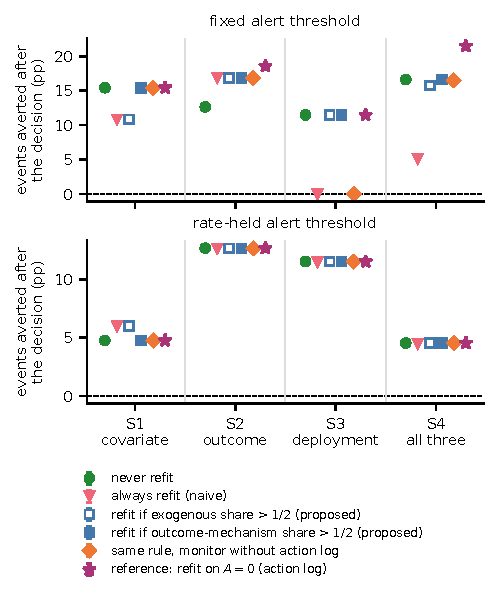
\includegraphics[width=\columnwidth]{figures/fig6_decision.pdf}
\caption{Keep-or-refit rules. Events averted against standard care in the
window after the decision, by scenario, under the fixed alert threshold (top)
and the rate-held threshold (bottom). Points are means over 200 independent
replicates per scenario, with 95\% bootstrap intervals over replicates (most
are smaller than the markers). Open square: refit when the
exogenous share exceeds one half; filled square: refit when the
outcome-mechanism share exceeds one half; diamond: the same rule driven by the
monitor without action logs.}\label{fig:decision}\end{figure}
Each replicate draws pre-deployment and monitoring-window samples of $20{,}000$
patients (the monitoring window of S3 and S4 includes the $30\%$ randomised
unalerted arm), computes the two attributions, refits naively on the deployed
arm of the monitoring window, fits the reference refits, and evaluates each
choice on $40{,}000$ patients from the next window. The rules driven by the
oracle decomposition (in \texttt{merged\_expE1.json}) show that the loss of the
exogenous-share rule in S1 is a property of the rule, not of estimation error:
driven by the oracle it also refits in S1.

% generated by sim2/make_tables.py; do not edit by hand
\begin{table}[h]
\centering\scriptsize
\setlength{\tabcolsep}{3pt}
\caption{Keep-or-refit rules under the rate-held threshold (events averted, pp) and harm sensitivity under the fixed threshold: net events averted when each extra treatment of a patient whose untreated outcome is 0 costs $h$ events.}
\label{tab:decision-app}
\resizebox{\columnwidth}{!}{%
\begin{tabular}{llrrrr}
\toprule
Threshold & Rule & S1 & S2 & S3 & S4\\
\midrule
rate-held & Never refit & 4.77 & 12.70 & 11.55 & 4.55\\
rate-held & Always refit (naive) & 6.01 & 12.67 & 11.54 & 4.49\\
rate-held & Refit if exogenous share $>1/2$ & 6.01 & 12.67 & 11.55 & 4.55\\
rate-held & Refit if outcome share $>1/2$ & 4.77 & 12.67 & 11.55 & 4.55\\
rate-held & \quad same, monitor (no action log) & 4.77 & 12.67 & 11.54 & 4.55\\
rate-held & Reference: refit on $A{=}0$ & 4.77 & 12.70 & 11.55 & 4.55\\
\midrule
fixed, $h=0.1$ & Never refit & 14.3 & 12.0 & 10.5 & 15.8\\
fixed, $h=0.1$ & Always refit (naive) & 10.2 & 15.8 & 0.0 & 5.0\\
fixed, $h=0.1$ & Refit if exogenous share $>1/2$ & 10.2 & 15.8 & 10.5 & 15.0\\
fixed, $h=0.1$ & Refit if outcome share $>1/2$ & 14.3 & 15.8 & 10.5 & 15.8\\
fixed, $h=0.1$ & \quad same, monitor (no action log) & 14.3 & 15.8 & 0.0 & 15.7\\
fixed, $h=0.1$ & Reference: refit on $A{=}0$ & 14.3 & 17.3 & 10.5 & 20.2\\
fixed, $h=0.2$ & Never refit & 13.1 & 11.4 & 9.6 & 15.1\\
fixed, $h=0.2$ & Always refit (naive) & 9.5 & 14.7 & 0.0 & 4.8\\
fixed, $h=0.2$ & Refit if exogenous share $>1/2$ & 9.5 & 14.7 & 9.6 & 14.3\\
fixed, $h=0.2$ & Refit if outcome share $>1/2$ & 13.1 & 14.7 & 9.6 & 15.1\\
fixed, $h=0.2$ & \quad same, monitor (no action log) & 13.1 & 14.7 & 0.0 & 15.0\\
fixed, $h=0.2$ & Reference: refit on $A{=}0$ & 13.1 & 16.0 & 9.6 & 18.9\\
\bottomrule
\end{tabular}
}
\end{table}


\begin{figure*}[t]\centering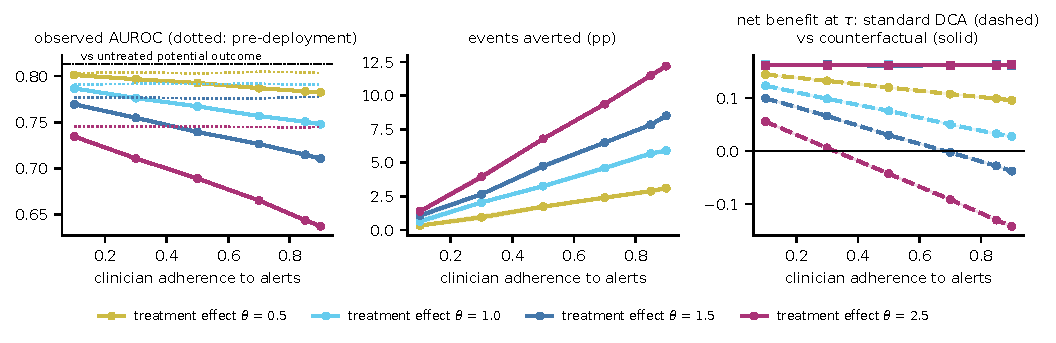
\includegraphics[width=\textwidth]{figures/fig5_utility.pdf}
\caption{Observed AUROC, events averted, and standard versus counterfactual
net benefit across clinician adherence and treatment effect $\theta$, S3
operating point otherwise. Means over 20 independent replicates per cell;
95\% bootstrap bands of the mean are mostly narrower than the lines.}\label{fig:utility}\end{figure*}
\section{Intervals, coverage and harm}
\label{app:intervals}
The numbers for Experiments A, B, D, E and F in Section~\ref{sec:sim} come
from a rerun with one seed block per row that stores every replicate
(\texttt{merged\_expE7.json}); bracketed intervals are 95\% percentile
bootstrap intervals of the mean over replicates. They measure Monte Carlo
error. To show what an analyst would report from one dataset, every replicate
of A and B also gets a patient-level bootstrap (300 resamples;
pre-deployment patients resampled, post-deployment patients resampled within
randomised arm). The proposed decomposition's intervals cover its own estimand in $90\%$ to $99\%$ of replicates for every non-degenerate term in S1 to S4 (Table~\ref{tab:coverage}), all but one within the range a nominal $95\%$ gives with 100 replicates (about $91\%$ to $99\%$), and the policy term in $93\%$ to $100\%$ at every $\varepsilon$ (Table~\ref{tab:positivity-ci}). The monitor's intervals cover the marginal game it estimates at similar rates ($88\%$ to $99\%$) but never cover the policy-contrast outcome term in S3 or S4: the analyst sees a tight, well-calibrated interval for the wrong estimand. The unclipped union-graph estimator's intervals are 4.4 to 4.7 times wider than the proposed ones and cover their target in $87\%$ (S3) and $80\%$ (S4) of replicates; clipped, they never cover it. At $\varepsilon = 0$ the union-graph interval excludes the target at every sample size and narrows as $n$ grows.

% generated by sim2/make_tables_e7.py; do not edit by hand
\begin{table}[h]
\centering\scriptsize
\setlength{\tabcolsep}{3pt}
\caption{Analyst-facing intervals. Share of replicates (\%) whose 95\% patient-level bootstrap interval (300 resamples) covers the estimator's own estimand, with the median interval width in Brier units, over 100 independent replicates per scenario ($n=20{,}000$ per environment). One row scores the monitor against the policy-contrast outcome term, the target a refit decision needs. ``exact'': the term is identically zero when nothing is deployed.}
\label{tab:coverage}
\resizebox{\columnwidth}{!}{%
\begin{tabular}{lcccc}
\toprule
Estimator and term & S1 & S2 & S3 & S4\\
\midrule
Proposed $X$ & 93 (0.006) & 92 (0.002) & 90 (0.003) & 97 (0.007)\\
Proposed $Y$ & 99 (0.010) & 95 (0.008) & 93 (0.013) & 94 (0.015)\\
Proposed $\pi$ & exact & exact & 95 (0.014) & 95 (0.015)\\
Monitor $X$ & 93 (0.006) & 92 (0.002) & 88 (0.004) & 97 (0.006)\\
Monitor $Y|X$ & 99 (0.010) & 94 (0.008) & 93 (0.009) & 95 (0.012)\\
Monitor $Y|X$ vs.\ policy-contrast $Y$ & 99 (0.010) & 95 (0.008) & 0 (0.009) & 0 (0.012)\\
Union graph $\pi$, unclipped & exact & exact & 87 (0.063) & 80 (0.065)\\
Union graph $\pi$, clipped & exact & exact & 0 (0.011) & 0 (0.010)\\
\bottomrule
\end{tabular}
}
\end{table}

% generated by sim2/make_tables_e7.py; do not edit by hand
\begin{table}[h]
\centering\scriptsize
\setlength{\tabcolsep}{3pt}
\caption{Positivity continuum and sample size. Top: coverage (\%) of the 95\% patient-level bootstrap interval for the policy term, S3 operating point. Bottom: union-graph estimate at $\varepsilon=0$ against its target, with the median analyst interval; the interval narrows around a value of the wrong sign.}
\label{tab:positivity-ci}
\begin{tabular}{lccc}
\toprule
$\varepsilon$ & Union, unclipped & Union, clipped & Proposed\\
\midrule
0 & 0 & 0 & 100\\
0.0001 & 33 & 0 & 93\\
0.001 & 83 & 0 & 93\\
0.01 & 97 & 97 & 100\\
0.05 & 97 & 97 & 93\\
\midrule
$n$ & Estimate & Median 95\% interval & Covers target\\
\midrule
20{,}000 & $-$0.0091 & [$-$0.0102, $-$0.0077] & 0\%\\
50{,}000 & $-$0.0086 & [$-$0.0094, $-$0.0079] & 0\%\\
100{,}000 & $-$0.0088 & [$-$0.0094, $-$0.0083] & 0\%\\
200{,}000 & $-$0.0087 & [$-$0.0091, $-$0.0084] & 0\%\\
400{,}000 & $-$0.0088 & [$-$0.0091, $-$0.0085] & 0\%\\
\midrule
\multicolumn{4}{l}{Target (oracle Shapley policy term): 0.0269}\\
\bottomrule
\end{tabular}
\end{table}


\emph{Harm for unnecessary treatment.} Events averted count only benefit.
Charging each extra treatment given to a patient whose untreated outcome is 0
a harm of $h$ events gives the net figures of Table~\ref{tab:harm}.
At the S3 operating point with adherence $0.85$ the alert policy averts $11.50$ points; with $h = 0.05$, $0.1$ and $0.2$ the net figures are $11.03$, $10.56$ and $9.63$. The update-rule comparison is unchanged by the penalty (naive refitting's net benefit stays near zero while keeping the score loses the same fraction as the policy). The same penalty leaves the ranking of keep-or-refit rules unchanged for
$h \le 0.2$ (Table~\ref{tab:decision-app}).

% generated by sim2/make_tables_e7.py; do not edit by hand
\begin{table}[h]
\centering\scriptsize
\setlength{\tabcolsep}{4pt}
\caption{Harm sensitivity. Net events averted by the alert policy against standard care (percentage points) when each extra treatment of a patient whose untreated outcome is 0 costs $h$ events; $\theta = 2.5$, mean over 20 independent replicates per cell; 95\% bootstrap intervals are within $\pm0.05$.}
\label{tab:harm}
\begin{tabular}{lcccc}
\toprule
Adherence & $h=0$ & $h=0.05$ & $h=0.1$ & $h=0.2$\\
\midrule
0.1 & 1.34 & 1.28 & 1.23 & 1.12\\
0.3 & 4.03 & 3.87 & 3.70 & 3.37\\
0.5 & 6.75 & 6.48 & 6.20 & 5.65\\
0.7 & 9.45 & 9.07 & 8.68 & 7.91\\
0.85 & 11.50 & 11.03 & 10.56 & 9.63\\
0.9 & 12.21 & 11.71 & 11.22 & 10.22\\
\bottomrule
\end{tabular}
\end{table}


\section{Semi-synthetic MIMIC-IV experiment}
\label{app:mimic}
\emph{Cohort.} Adult ward inpatients in MIMIC-IV~\citep{johnson2023mimic},
version 3.1~\citep{johnson2024mimiciv}, from
PhysioNet~\citep{goldberger2000physionet}.
One prediction time per admission, drawn at random among creatinine draws
taken on a ward at least four hours after admission and outside any ICU
stay. A ward is a care unit that is not an intensive care, emergency,
recovery, obstetric, newborn, psychiatric, discharge-lounge or unknown unit,
and in which ICU stays begin for fewer than $10\%$ of admissions and
transfers; this excludes two neurological step-down units, in which most do,
but not the general wards on which MIMIC-IV records a handful of ICU stays. Features: age, sex, emergency admission, hours since admission, a
prior ICU stay in the same admission, and the last value in the preceding
24 hours of creatinine, urea nitrogen, sodium, potassium, chloride,
bicarbonate, glucose, anion gap, white cells, haemoglobin and platelets, with
missing indicators. Outcome: ICU admission or in-hospital death within
12 hours. Pre-deployment period: patients with anchor year group 2008--2013;
post-deployment period: 2014--2019.
\emph{Simulated components.} The score is a logistic regression fitted to
$40\%$ of early-period patients; alerts fire at a $10\%$ alert rate on those
patients; an alert is acted upon with probability $0.85$; an acted-upon alert
prevents an event that would otherwise occur with probability $0.5$ and never
causes one; $30\%$ of post-deployment patients form a randomised unalerted
arm; the refit loop runs for eight rounds, each refit on a bootstrap sample
of the whole post-deployment training pool, since at an event rate near
$1\%$ a smaller sample holds too few events for 24 features.
Everything else, including the outcome under standard care, is observed.
\emph{Targets.} The policy contrast and the total exogenous change are known
for the finite pools in expectation over the simulated components; the split
of the exogenous change into covariate and outcome parts has no ground truth
in real data and is reported, not scored.

\emph{Results.} Table~\ref{tab:mimic} and Figure~\ref{fig:mimic} give the
main run and Table~\ref{tab:mimic-sens} the sensitivity runs; everything was
computed on the machine that holds the data, and only these aggregates left
it. The cohort has $368{,}995$ ward admissions of $155{,}852$ patients:
$229{,}280$ in 2008--2013, $110{,}093$ in 2014--2019 and $29{,}622$ in
2020--2022, used only in the run with that late period; $30\%$ of prediction
times are on general medicine wards. ICU admission within 12 hours follows
$0.89\%$ of prediction times and death $0.05\%$. The score is fitted to
$91{,}002$ early-period admissions; its AUROC is $0.747$ on the held-out early
admissions and $0.723$ in the late period, and its threshold, a predicted risk
of $0.016$, flags $9.9\%$ and $10.4\%$ of them.

\emph{Performance drop.} On the held-out early admissions the deployment
lowers the Brier score from $0.0083$ to $0.0070$, AUROC from $0.747$ to
$0.702$, observed over expected events from $1.04$ to $0.87$ and the
calibration slope from $1.05$ to $0.83$ (\texttt{performance\_drop.json}). In
the late period the score under-predicts under historical care (observed over
expected $1.27$; the event rate has risen), and the same deployment brings the
ratio to $1.07$: the alert's benefit hides the calibration drift as well as
the rise in the Brier score.

\emph{Precision.} The randomised arm recovers the policy term in every run.
Its bias intervals cover zero in 13 of the 14 runs and scenarios; the
exception, periods by admission year with drift, is $-0.00012$ [$-0.00023$,
$-0.00001$], $8\%$ of the term. One analyst's estimate is imprecise: its
single-run SD is $0.0005$ to $0.0006$ in every scenario except drift and
deployment with 2020--2022 as the late period ($0.0013$ with $29{,}622$
admissions), three quarters of the term when the action prevents a quarter of
events.

\emph{Masking.} With real drift and deployment, the observed change in the
Brier score is $+0.00039$ in the main run and $+0.00108$ when the action
prevents a quarter of events, against a real deterioration of $+0.00190$; it
is $-0.00038$ when the action prevents three quarters and $-0.00023$ when the
alert flags $20\%$ of patients, so the deterioration then looks like an
improvement.

\emph{Union graph.} Every pre-deployment patient has $A = 0$, so the oracle
policy weight is $0.15$ for alerted and $1$ for other patients, and the
estimate measures how the alerted patients' losses enter the average, not what
the action does: it is identical, replicate by replicate, whether the action
prevents $25\%$, $50\%$ or $75\%$ of events, against policy contrasts from
$-0.00064$ to $-0.00191$.

\emph{Split of the real drift.} The total exogenous change is recovered in
every run, within $0.00012$ of its target. Its split into covariate and
outcome terms rests on a classifier's density ratio between the periods and is
not stable: in the main run the two terms have single-run SDs of $0.0018$ and
$0.0019$, as large as the total, $+0.0019$ (means $+0.0030$ for $P(X)$ and $-0.0011$ for
the outcome mechanism without deployment), and with periods by admission year
or 2020--2022 as the late period the two terms reach $\pm 0.01$ to
$\pm 0.03$, with single-run SDs of the same size. The monitor and the proposed
decomposition share the ratio and the problem; the policy term and the total
need no ratio.

\emph{Update rules.} Under the fixed threshold, refitting on untreated
patients averts more events than naive refitting in every run, by $0.005$ to
$0.079$ points, the difference growing with the action's effect. Both refits
recalibrate to the late period and flag more patients than the kept score, so
whether naive refitting beats keeping the score depends on whether that gain
exceeds what the prevented events cost ($-0.044$ to $+0.037$ points). With
the alert rate held, the two refits are within $0.006$ points of each other in
every run and within $0.024$ points of the kept score, usually below it: every
refit learns from post-deployment data in which most alerted patients were
treated. The weighted refit is within $0.013$ points of the unweighted one in
every run.

\emph{Periods.} Anchor year groups date an admission only to within several
years. With periods by admission year, which drops admissions whose
three-year window straddles 2013 and 2014, the early and late periods hold
$127{,}323$ and $125{,}683$ admissions, and the conclusions above hold. With
2020--2022 as the late period ($29{,}622$ admissions, event rate $1.13\%$) the
policy term and the exogenous change are recovered with wider intervals.

\IfFileExists{tables/e6_mimic.tex}{% generated by sim2/make_tables.py; do not edit by hand
\begin{table*}[t]
\centering\scriptsize
\caption{Semi-synthetic MIMIC-IV. Cohort: 368{,}995 ward admissions of 155{,}852 adult patients, of which 229{,}280 in 2008--2013 (event rate 0.8\%) and 110{,}093 in 2014--2019 (1.0\%); score AUROC 0.747 on held-out early patients and 0.723 in the late period; alert rate 10.4\% in the late period at the fixed threshold. Top: attribution of the Brier-score change, mean over 200 replicates with 95\% bootstrap intervals; targets are exact for the cohort in expectation over the simulated components. Bottom: events averted against historical care at round 8 (percentage points), 50 replicates.}
\label{tab:mimic}
\begin{tabular}{lccc}
\toprule
 & Deployment only & Drift only & Drift and deployment\\
\midrule
Policy contrast (target) & $-$0.00127 & 0 & $-$0.00147\\
Proposed, policy term & $-$0.00131 [$-$0.00138, $-$0.00124] & 0 & $-$0.00154 [$-$0.00162, $-$0.00146]\\
Union graph, oracle weights & $-$0.00215 [$-$0.00217, $-$0.00214] & -- & --\\
Monitor, $P(Y\mid X)$ & $-$0.00128 [$-$0.00133, $-$0.00123] & $-$0.00113 [$-$0.00141, $-$0.00088] & $-$0.00244 [$-$0.00272, $-$0.00216]\\
Exogenous change (target) & 0 & $+$0.00190 & $+$0.00190\\
Proposed, exogenous terms & $+$0.00003 [$-$0.00004, $+$0.00009] & $+$0.00187 [$+$0.00181, $+$0.00192] & $+$0.00193 [$+$0.00186, $+$0.00201]\\
Observed change in Brier score & $-$0.00129 & $+$0.00187 & $+$0.00039\\
Observed change in AUROC & $-$0.044 & $-$0.022 & $-$0.068\\
\midrule
Update rule, round 8 & Fixed threshold & Rate-held threshold & \\
\midrule
Keep & 0.154 & 0.154 & \\
Naive refit & 0.148 [0.145, 0.152] & 0.145 [0.144, 0.147] & \\
Refit on $A{=}0$ & 0.177 [0.173, 0.181] & 0.143 [0.141, 0.144] & \\
Refit on $A{=}0$, weighted & 0.183 [0.178, 0.187] & 0.144 [0.142, 0.146] & \\
\bottomrule
\end{tabular}
\end{table*}
}{}
\IfFileExists{tables/e6_sensitivity.tex}{% generated by sim2/make_tables.py; do not edit by hand
\begin{table*}[t]
\centering\scriptsize
\caption{Semi-synthetic MIMIC-IV, sensitivity runs. Deployment-only attribution (policy contrast, its randomised-arm estimate, the union-graph estimate with oracle policy weights and the monitor's $P(Y\mid X)$ term, Brier units) and events averted at the last round under the fixed threshold (percentage points). Means with 95\% bootstrap intervals over replicates (the union-graph intervals are narrower than the last digit); the main analysis uses an alert rate of 10\%, an action that prevents the event with probability 0.5 and periods by anchor year group.}
\label{tab:mimic-sens}
\resizebox{\textwidth}{!}{%
\begin{tabular}{lccccccc}
\toprule
Setting & Policy contrast & Proposed $\pi$ & Union graph & Monitor $P(Y\mid X)$ & Keep & Naive refit & Refit on $A{=}0$\\
\midrule
Main analysis & $-$0.00127 & $-$0.00131 [$-$0.00138, $-$0.00124] & $-$0.00215 & $-$0.00128 [$-$0.00133, $-$0.00123] & 0.154 & 0.148 [0.145, 0.152] & 0.177 [0.173, 0.181]\\
Action prevents the event w.p.\ 0.25 & $-$0.00064 & $-$0.00068 [$-$0.00077, $-$0.00059] & $-$0.00216 & $-$0.00065 [$-$0.00073, $-$0.00057] & 0.077 & 0.083 [0.082, 0.085] & 0.089 [0.086, 0.091]\\
Action prevents the event w.p.\ 0.75 & $-$0.00191 & $-$0.00194 [$-$0.00204, $-$0.00186] & $-$0.00216 & $-$0.00192 [$-$0.00199, $-$0.00185] & 0.231 & 0.188 [0.178, 0.197] & 0.266 [0.258, 0.274]\\
Alert rate 5\% & $-$0.00090 & $-$0.00094 [$-$0.00104, $-$0.00085] & $-$0.00165 & $-$0.00091 [$-$0.00099, $-$0.00084] & 0.101 & 0.104 [0.100, 0.108] & 0.122 [0.117, 0.126]\\
Alert rate 20\% & $-$0.00178 & $-$0.00182 [$-$0.00192, $-$0.00174] & $-$0.00279 & $-$0.00180 [$-$0.00186, $-$0.00173] & 0.225 & 0.210 [0.205, 0.215] & 0.252 [0.245, 0.259]\\
Periods by admission year & $-$0.00126 & $-$0.00128 [$-$0.00140, $-$0.00116] & $-$0.00213 & $-$0.00136 [$-$0.00144, $-$0.00127] & 0.161 & 0.139 [0.136, 0.141] & 0.167 [0.163, 0.170]\\
Late period 2020--2022 & $-$0.00127 & $-$0.00131 [$-$0.00141, $-$0.00122] & $-$0.00216 & $-$0.00128 [$-$0.00135, $-$0.00121] & 0.173 & 0.209 [0.202, 0.216] & 0.233 [0.224, 0.243]\\
\bottomrule
\end{tabular}
}
\end{table*}
}{}

\section{Proofs}
For a binary outcome, write $\ell_y(x) = \ell(f(x), y)$; for the Brier score
$\ell_1 - \ell_0 = 1 - 2f(x)$.

\emph{Proposition~\ref{prop:absence}.} Let
$g_0(x) = P_{e_0}(Y{=}1 \mid X = x, A = a)$ on $\mathcal{X}_a$. Because
$\pi_0(a \mid x) = 0$ there, the distribution of $(X, A, Y)$ in $e_0$ does not
depend on $g_0$, and the distribution in $e_1$ depends only on the
post-deployment outcome mechanism; processes that differ only in $g_0$ give the
same data. A coalition $S$ with $m_A \in S$ and $m_Y \notin S$ puts mass
$p_S(x)\, \pi_1(a \mid x, f(x)) > 0$ on $(x, a)$, $x \in \mathcal{X}_a$, where
$p_S$ is the covariate density of the period that supplies $P(X)$, and its
expected loss there is $\ell_0(x) + g_0(x)\{\ell_1(x) - \ell_0(x)\}$. A
perturbation $\delta$ of $g_0$ therefore changes $v(S)$ by
$\int_{\mathcal{X}_a} p_S\, \pi_1\, (\ell_1 - \ell_0)\, \delta\, dx$, and the
weights $\pi_1/\pi_0$ are infinite on $\mathcal{X}_a$. Shapley values are linear
in $v$. With three players, $\{m_A\}$ and $\{m_A, P(X)\}$ enter $\phi_{m_A}$
with weights $1/3$ and $1/6$ and $\phi_{m_Y}$ with weights $-1/6$ and $-1/3$;
choosing $\delta$ with the sign of $\ell_1 - \ell_0$ moves both coalition values
the same way, so neither Shapley value is identified. The only non-identified
term of $\phi_{P(X)}$ is $\frac{1}{6}\{v(\{P(X), m_A\}) - v(\{m_A\})\}$, which
changes by
$\frac{1}{6} \int_{\mathcal{X}_a} (p_{e_1} - p_{e_0})\, \pi_1\,
(\ell_1 - \ell_0)\, \delta\, dx$; this vanishes for every $\delta$ only if
$p_{e_1} = p_{e_0}$ almost everywhere on the part of $\mathcal{X}_a$ where
$\ell_1 \neq \ell_0$. Assuming the outcome mechanism unchanged on
$\mathcal{X}_a$ sets $g_0$ equal to its post-deployment value, which $e_1$
identifies. $\square$

\emph{Proposition~\ref{prop:misattr}.} With $P(X)$ unchanged, switching only
$P(X)$ reproduces $e_0$ and switching only $P(Y \mid X)$ reproduces $e_1$, so
$v(\{P(X)\}) = 0$ and $v(\{P(Y \mid X)\}) = v(\mathcal{M}') = \Delta R$. Then
$\phi_{P(X)} = \frac12\{v(\{P(X)\}) - v(\emptyset)\} +
\frac12\{v(\mathcal{M}') - v(\{P(Y \mid X)\})\} = 0$, and by efficiency
$\phi_{P(Y \mid X)} = \Delta R$. The risk reduction on the alerted region makes
$P_{e_1}(Y \mid X) \neq P_{e_0}(Y \mid X)$ there, so the whole change is the
policy's. $\square$

\emph{Proposition~\ref{prop:rd}.} The policies agree below $\tau$, so
$\E[Y \mid \rhat = r] = \E[Y(\pi_0) \mid \rhat = r]$ for $r < \tau$ and
$\E[Y(\pi_0) \mid \rhat = r] + \theta(r)$ for $r \geq \tau$; with
$\E[Y(\pi_0) \mid \rhat = r]$ continuous at $\tau$, the jump is the right limit
of $\theta$ at $\tau$, written $\theta(\tau)$. $\Theta$ integrates the policy's
effect over $F$. For a prediction $r$ and binary $Y$,
$(r - Y)^2 = r^2 + (1 - 2r) Y$, so
$\Delta_\pi = \E[(1 - 2\rhat)\{Y(\pi_1) - Y(\pi_0)\}] =
\int_{r \geq \tau} (1 - 2r)\, \theta(r)\, dF(r)$. Nothing in the jump constrains
$\theta$ on $(\tau, 1]$, so neither quantity is identified without a
restriction. Case (a) is immediate. In case (b), $|\theta(r)| \geq
|\theta(\tau)|$ for $r \geq \tau$ when $|\theta|$ is nondecreasing, so
$|\Theta| \geq |\theta(\tau)|\, \bar F(\tau)$, and the inequality reverses when
$|\theta|$ is nonincreasing. $\square$

\emph{Proposition~\ref{prop:nonid}.} In both models of the example $P(X)$ is
the same in the two periods, $P_{e_1}(Y{=}1 \mid x) = P_{e_0}(Y{=}1 \mid x) -
\delta(x)\, \mathbb{1}\{f(x) \geq \tau\}$, and $\rhat = f(X)$ is a function of
$X$, so the observed distributions coincide. In the first model, standard care
in $e_1$ restores $P_{e_0}(Y \mid X)$, so $R_{e_1}(f; \pi_0) =
R_{e_0}(f; \pi_0)$ and $\Delta_\pi = \Delta R$; in the second,
$Y(\pi_0) = Y(\pi_1)$ for every patient, so $\Delta_\pi = 0$. $\square$

\end{document}
